%% (Master) Thesis template
% Template version used: v1.4
%
% Largely adapted from Adrian Nievergelt's template for the ADPS
% (lecture notes) project.


%% We use the memoir class because it offers a many easy to use features.
\documentclass[11pt,a4paper,titlepage]{memoir}

%% Packages
%% ========

%% LaTeX Font encoding -- DO NOT CHANGE
\usepackage[OT1]{fontenc}

%% Babel provides support for languages.  'english' uses British
%% English hyphenation and text snippets like "Figure" and
%% "Theorem". Use the option 'ngerman' if your document is in German.
%% Use 'american' for American English.  Note that if you change this,
%% the next LaTeX run may show spurious errors.  Simply run it again.
%% If they persist, remove the .aux file and try again.
\usepackage[english]{babel}

%% Input encoding 'utf8'. In some cases you might need 'utf8x' for
%% extra symbols. Not all editors, especially on Windows, are UTF-8
%% capable, so you may want to use 'latin1' instead.
\usepackage[utf8]{inputenc}

%% This changes default fonts for both text and math mode to use Herman Zapfs
%% excellent Palatino font.  Do not change this.
\usepackage[sc]{mathpazo}

%% The AMS-LaTeX extensions for mathematical typesetting.  Do not
%% remove.
\usepackage{amsmath,amssymb,amsfonts,mathrsfs}

%% NTheorem is a reimplementation of the AMS Theorem package. This
%% will allow us to typeset theorems like examples, proofs and
%% similar.  Do not remove.
%% NOTE: Must be loaded AFTER amsmath, or the \qed placement will
%% break
\usepackage[amsmath,thmmarks]{ntheorem}

%% LaTeX' own graphics handling
\usepackage[dvipsnames]{xcolor}
\usepackage{graphicx}

%% We unfortunately need this for the Rules chapter.  Remove it
%% afterwards; or at least NEVER use its underlining features.
\usepackage{soul}

%% This allows you to add .pdf files. It is used to add the
%% declaration of originality.
\usepackage{pdfpages}



%% Some more packages that you may want to use.  Have a look at the
%% file, and consult the package docs for each.
\input{extrapackages}

%% Our layout configuration.  DO NOT CHANGE.
\input{layoutsetup}

%% Theorem environments.  You will have to adapt this for a German
%% thesis.
\input{theoremsetup}


%% Make document internal hyperlinks wherever possible. (TOC, references)
%% This MUST be loaded after varioref, which is loaded in 'extrapackages'
%% above.  We just load it last to be safe.
% \usepackage[linkcolor=black,colorlinks=true,citecolor=black,filecolor=black]{hyperref}
\usepackage[colorlinks=true,citecolor=black]{hyperref}


%% Helpful macros.
%% Custom commands
%% ===============


\usepackage{minted}
\usepackage{xspace}
\usepackage{cleveref}
\usepackage{algorithm}
\usepackage{algpseudocode}
\usepackage{graphicx}
\usepackage{subcaption}
\usepackage{bm}
\usepackage{tikz}
\usepackage{rotating}
\usepackage{minitoc}
\usepackage{etoolbox}

% hopefully nice section coloring?
\usepackage{titlesec}

% make minitoc tocdpeth match tocdepth
% \setcounter{minitocdepth}{\value{tocdepth}}
% \setcounter{minitocdepth}{subsubsection}
\setcounter{minitocdepth}{3}

\titleformat{name=\section}[block]
  {\sffamily\Large\bfseries}
  {}
  {0pt}
  {\colorsectionblue}
\titlespacing*{\section}{0pt}{\baselineskip}{\baselineskip}

\titleformat{name=\subsection}[block]
  {\sffamily\bfseries}
  {}
  {0pt}
  {\colorsubsectiongreen}
\titlespacing*{\subsection}{0pt}{\parskip}{0pt}

\titleformat{name=\subsubsection}[block]
  {\sffamily\bfseries}
  {}
  {0pt}
  {\colorsubsubsectionred}
\titlespacing*{\section}{0pt}{\baselineskip}{\baselineskip}

\newcommand{\colorsectionblue}[1]{%
  \colorbox{blue!20}{\parbox{\dimexpr\textwidth-2\fboxsep}{\color{black}\thesection\ #1}}}

\newcommand{\colorsubsectiongreen}[1]{%
  \colorbox{green!20}{\parbox{\dimexpr\textwidth-2\fboxsep}{\color{black}\thesubsection\ #1}}}


\newcommand{\colorsubsubsectionred}[1]{%
\colorbox{red!20}{\parbox{\dimexpr\textwidth-2\fboxsep}{\color{black}\thesubsubsection\ #1}}}


\newcommand{\q}[1]{``#1''}


% GIRGs
\newcommand{\GIRG}{\mathrm{GIRG}}
\DeclareMathOperator{\shrinktogcc}{\textcolor{blue}{shrinkToGCC}}
\DeclareMathOperator{\uniformify}{\textcolor{blue}{uniformify}}
\newcommand{\PLP}{\mintinline{python}|powerlaw|\xspace}
\newcommand{\ffit}{f_{\mathrm{fit}}}  % statistic with which to fit GGM parameter
% statistic(s) with which to classify real/fake graphs
\newcommand{\fclass}{f^{\mathrm{class}}}  


%% Special characters for number sets, e.g. real or complex numbers.
\newcommand{\C}{\mathbb{C}}
\newcommand{\K}{\mathbb{K}}
\newcommand{\N}{\mathbb{N}}
\newcommand{\Q}{\mathbb{Q}}
\newcommand{\R}{\mathbb{R}}
\newcommand{\Z}{\mathbb{Z}}
\newcommand{\X}{\mathbb{X}}
\newcommand{\T}{\mathbb{T}}

% Brackets
\newcommand{\abs}[1]{\left\lvert #1\right\rvert}
\newcommand{\bket}[1]{\left\lvert #1\right\rangle}
\newcommand{\brak}[1]{\left\langle #1 \right\rvert}
\newcommand{\braket}[2]{\left\langle #1\middle\vert #2 \right\rangle}
\newcommand{\bra}{\langle}
\newcommand{\ket}{\rangle}
\newcommand{\norm}[1]{\left\lVert #1\right\rVert}
\newcommand{\normalorder}[1]{\mathop{:}\nolimits\!#1\!\mathop{:}\nolimits}
\newcommand{\tv}[1]{|#1|}
% \renewcommand{\vec}[1]{\boldsymbol{\mathbf{#1}}}
\renewcommand{\vec}[1]{\bm{#1}}
% Probability
\DeclareMathOperator{\Bernoulli}{Bernoulli}
\DeclareMathOperator{\betaD}{beta}
\DeclareMathOperator{\bias}{bias}
\DeclareMathOperator{\binomial}{binomial}
\DeclareMathOperator{\corr}{corr}
\DeclareMathOperator{\cov}{cov}
\DeclareMathOperator{\gammaD}{gamma}
\DeclareMathOperator{\mse}{mse}
\DeclareMathOperator{\multinomial}{multinomial}
\DeclareMathOperator{\Poisson}{Poisson}
\DeclareMathOperator{\var}{var}
\DeclareMathOperator{\powerlaw}{powerlaw}
\newcommand{\E}{\mathbb{E}}
\newcommand{\PP}{\mathbb{P}}

% Caligraphic
\newcommand{\cA}{\mathcal{A}}
\newcommand{\cB}{\mathcal{B}}
\newcommand{\cC}{\mathscr{C}}
\newcommand{\cD}{\mathcal{D}}
\newcommand{\cE}{\mathscr{E}}
\newcommand{\cF}{\mathcal{F}}
\newcommand{\cG}{\mathscr{G}}
\newcommand{\cH}{\mathcal{H}}
\newcommand{\cM}{\mathcal{M}}

% Other
\DeclareMathOperator*{\argmax}{arg\,max}
\DeclareMathOperator*{\argmin}{arg\,min}
\newcommand{\eqname}[1]{\tag*{#1}}% Tag equation with name



%% Fixed/scaling delimiter examples (see mathtools documentation)
% \DeclarePairedDelimiter\abs{\lvert}{\rvert}
% \DeclarePairedDelimiter\norm{\lVert}{\rVert}

%% Use the alternative epsilon per default and define the old one as \oldepsilon
\let\oldepsilon\epsilon
\renewcommand{\epsilon}{\ensuremath\varepsilon}

%% Also set the alternate phi as default.
% \let\oldphi\phi
% \renewcommand{\phi}{\ensuremath{\varphi}}



%% benji: try to color all math mode text
% \renewcommand{\displaymath}{\color{red}\[}
% \renewcommand{\enddisplaymath}{\]\@ignoretrue\color{black}}

\definecolor{byzantium}{rgb}{0.44, 0.16, 0.39}
\definecolor{darkred}{rgb}{0.55, 0.2, 0.0}
\definecolor{electricyellow}{rgb}{1.0, 1.0, 0.0}
\definecolor{amber}{rgb}{1.0, 0.75, 0.0}
\definecolor{awesome}{rgb}{1.0, 0.13, 0.32}
\definecolor{applegreen}{rgb}{0.5, 0.65, 0.0}

\everymath{\color{darkred}}

\AtBeginEnvironment{equation*}{\color{darkred}}
\AtBeginEnvironment{align*}{\color{darkred}}
\AtBeginEnvironment{equation}{\color{darkred}}
\AtBeginEnvironment{align}{\color{darkred}}

% \everydisplay\expandafter{\the\everydisplay \color{blue}}
% my tables are now math colored??
% unfortunately this fix then stops my align environments from working
% \makeatletter
% \def\m@th{\mathsurround\z@\color{black}}
% \makeatother

% Restore black color for tables
% \AtBeginEnvironment{tabular}{\color{black}}
% \AtBeginEnvironment{table}{\color{black}}

% % Reset color after tables
% \AtEndEnvironment{tabular}{\color{black}}
% \AtEndEnvironment{table}{\color{black}}

% my footnotes are now math colored too?
% \makeatletter
% \renewcommand\@makefnmark{\hbox{\@textsuperscript{\normalfont\color{red}\@thefnmark}}}
% \makeatother
\renewcommand\thefootnote{\textcolor{green}{\arabic{footnote}}}


% make italics a different color
\let\oldtextit\textit 
\renewcommand\textit[1]{\oldtextit{\color{applegreen}#1}}

% color links?
\hypersetup{colorlinks,linkcolor=awesome}

%% benji: make subsubsection also count?
% \setcounter{tocdepth}{3}
% \setcounter{secnumdepth}{3}

%% Document information
%% ====================

\title{GIRG model for realistically generating social network graphs}
\author{Benjamin Dayan}
\thesistype{Master Thesis}
\advisors{Advisors: Prof.\ Dr.\ Angelika Steger, Prof.\ Dr.\ Johannes Lengler, Marc Kauffman, Ulysse Schaller}
\department{Department of Computer Science}
\date{August 30, 2023}



%% benji: make margins bigger hopefully?

\setlrmarginsandblock{4.0cm}{3.0cm}{*}
\setulmarginsandblock{3.0cm}{*}{1}
\checkandfixthelayout 

%% benji: fix strange bug?

% \let\displaystyle\textstyle


% \def\MT@set@inh@list#1#2{%
%   \MT@ifempty\MT@inh@feat{%
%     \MT@map@clist@c\MT@features{\begingroup % <--
%       \MT@ifstreq{##1}{tr}\relax{\MT@declare@char@inh{##1}{#1}{#2}}%
%     \endgroup}% <--
%   }{%
%     \MT@map@clist@c\MT@inh@feat{\begingroup % <--
%       \KV@@sp@def\@tempa{##1}%
%       \MT@ifempty\@tempa\relax{%
%         \edef\@tempa{\csname MT@rbba@\@tempa\endcsname}%
%         \MT@ifstreq\@tempa{tr}\relax{%
%           \MT@exp@one@n\MT@declare@char@inh{\@tempa}{#1}{#2}}}%
%     \endgroup}% <--
%   }%      
%   \MT@end@catcodes
% }       

\begin{document}

\let\displaystyle\textstyle


\frontmatter

%% Title page is autogenerated from document information above.  DO
%% NOT CHANGE.
\begin{titlingpage}
  \calccentering{\unitlength}
  \begin{adjustwidth*}{\unitlength-24pt}{-\unitlength-24pt}
    \maketitle
  \end{adjustwidth*}
\end{titlingpage}

%% The abstract of your thesis.  Edit the file as needed.
\begin{abstract}
  Real world graphs, in particular social networks, exhibit clustering and are proposed to have an underlying geometrical generative structure.
  The GIRG generative graph model is one such proposed geometric model. We show good capability of different GIRG variants to produce graphs resembling a dataset of real social network graphs in a range of high level graph features.
  We then explore practical methods of fitting GIRG node geometric location parameters to an input graph. Using this we show that low dimensional GIRGs are capable of a good amount of replication on a node and edge level of our social network graphs. Throughout we hope to provide guidance on methods in how to generate and fit different types of GIRG, as well as an intuitive understanding of the GIRG model.
\end{abstract}


%% TOC with the proper setup, do not change.
\cleartorecto
\dominitoc
\tableofcontents
\adjustmtc  % shift confused minitoc to be correct.
\mainmatter

%% Your real content!
% \input{introduction}
% \input{rules}
% \input{typography}

\chapter{GIRG generation}
\section{GIRGs definition}
We outline the key elements of GIRGs and the main variations and how they fit into a wider context of random graph models.

The GIRG definition according to \cite{bringmann2019geometric} is a random graph model defined by the edge connection probabilities

TODO below (div by n, infty norm) is what I had before, but in fact bringmann2019geometric uses below with div by W and ambiguous norm.
\begin{equation}
    p_{uv} = \Theta \left ( \min \left \{ 
        1,
        c \left (
            \frac{w_u w_v}{ n \norm{x_u - x_v}_\infty^d}
        \right )^\alpha    
    \right \}
    \right )
\end{equation}

\begin{equation}
    p_{uv} = \Theta \left ( \min \left \{ 
        1,
        c \left (
            \frac{w_u w_v / W}{\norm{x_u - x_v}^d}
        \right )^\alpha    
    \right \}
    \right )
\end{equation}

where $(w_u)_{u \in V}$ are node specific weights and $(x_u \in \chi)_{u \in V}$ are positions in some geometric space $\chi$, generally taken to be the d-dimensional torus or cube of side length 1.

This edge probability has a geometric factor from the distance $r_{uv} = \norm{x_u - x_v}_\infty$, and is proportional to $r_{uv}^{-d \alpha}$, where $\alpha > 0$, meaning that close by nodes are more likely to be connected. The $n^{-1}$ normalising factor ensures that as $n \to \infty$, expected node degrees are unchanged.

We often write $\rho_{uv} = \left ( \frac{w_u w_v / W}{\norm{x_u - x_v}^d} \right )$ to save on writing.

\paragraph{power law degree sequence} Like Chung-Lu, the weight sequences are usually assumed to follow a powerlaw distribution with an exponent $\tau \in (2, 3)$ (at least within some tolerance and in the large weight tail).
\begin{align*}
\eqname{exact power law distribution}
& W \sim \powerlaw(\tau)
\\
\eqname{pdf (default $x_{\min } = 1$)}
& p(w) = w^{-\tau} \text{ for } w \in [x_{\min }, \infty]
\\
& p(W \geq w) \propto w^{1 - \tau}
\end{align*}
% A general In practice a power law degree sequence is required to have a looser version of $\# \{w_u | w_u \geq w\} = \Theta(w^{1 - \tau})$.
This is a heavy tailed distribution (heavier than exponentially decaying tails). $\tau > 2$ is important to ensure that $E[W] = \Theta(1)$. This means that although we may in a sequence of $w_1, ..., w_n$ have some very large $w_i$, still the majority of the total weight is in the small valued $w_i$'s. 


\paragraph{Similarity to Chung-Lu} A key property of the GIRG model is that marginalising over possible node locations gives that $E_{x_v}[p_{uv} | x_u, w_u, w_v] = \Theta(\min\{1, \frac{w_u w_v}{n} \})$, which matches the Chung-Lu GGM. This means that many results for Chung-Lu carry through automatically into GIRGs, like simple facts that $E[d_u] = \Theta(w_u)$ (the expected degree of a node of a fixed weight is proportional to that weight). For this to hold we actually need to have $\alpha > 1$ - otherwise there are too many long distance edges. Essentially $\alpha > 1$ depresses the number of long distance edges to be $\Theta(\min\{1, \frac{w_u w_v}{W} \})$. No matter how large $\alpha$ is, there will always be $\Theta(\min\{1, \frac{w_u w_v}{W} \})$ short distance edges: $u \sim v$ where $p_{uv} = 1$.

\paragraph{Geometry} The exact geometry $\chi$, and the distance function $\norm{\cdot}$ can vary a great deal without affecting the key properties of GIRGs. $\chi = \T_d$ the d-dimensional torus is very handy for proofs, as the viewpoint of any node $x_u$ is equivalently at the "centre" of the space. For real applications the d-dimensional cube $\chi = [0, 1]^d$ can be more realistic, but then if $x_u$ is at the edge of the cube it has a different viewpoint to a node more at the centre of the cube.

Taking $\norm{\cdot} = \norm{\cdot}_\infty$ is also useful, but can be replaced equivalently by euclidean or other norms. The minimum component distance $\norm{x} = \min_i |x_i|$ is not a norm, but still holds retains most of the GIRG properties. This can make sense in that two nodes might have a higher edge probability by being close in one dimension, rather than every dimension.

The reason for the power of $d$ in $r_{uv}^d$ is to keep the edge probabilties equivalent with respect to the volume of space in different dimensions. The more general formula replaces replaces $||x_u - x_v||^d = r_{uv}^d$ with $Vol(B_r)$ the volume of the ball of radius $r=r_{uv}$.
For norms, $Vol(B_r) = \Theta(r^d)$, e.g. in the $\infty$-norm, $Vol(B_r) = (2r)^d$ as a cube with side-length $2r$. The euclidean ball has some $\pi$'s in the formula. For the minimum component distance, $Vol(B_r) = \Theta(r)$. Volumetric equivalence makes sense in that the edge probability $p_{uv} | x_u, w_u, w_v$ in the Torus is determined by integrating $\int_{r=0}^{r=1} p_{uv}(r) p(r) dr = \int_{Vol=0}^{Vol=1} p_{uv}(Vol) dVol$, where $Vol(r) = Vol(B_r)$ is the volume of the ball of radius $r$. Hence across different GIRGs of different dimensions $d$, keeping $p_{uv}(Vol)$ the same function therefore keeps the pairwise edge probabilities $p_{uv}$ the same (but not the joint edge probability distribution of course).




\section{C++ GIRGs}
We use the C++ implementation of GIRG generation by \cite{blasius2022efficiently}.
They implement the algorithm in \cite{bringmann2019geometric}, which they claim to have linear runtime.
A GIRG, having power law weighted nodes, is shown to have $\Theta(1)$ average degree.
Hence there are $\Theta(n)$ edges, so presumably this means that the runtime is not much different from an oracle writing out the edges sequentially.

We use this code so much so will need to take note of their preferred notation:
\begin{equation}
    p_{uv} = \min \left \{ 
        1,
        c \left (
            \frac{w_u w_v / W}{\norm{x_u - x_v}_\infty^d}
        \right )^\alpha    
    \right \}
\end{equation}
Where they take $x_u \in \chi = \T_d$ the torus. They use a variant of the GIRG where normalisation by $n$ is replaced by that of $W = \sum_{u \in V} w_u$. For $w_u$ obeying a $\tau > 2$ power law distribution, $W = \Theta(n)$ with high probability, so this is fine.

The inner constant $c$ in the C++ implementation still falls into the wider GIRG definition of $p_{uv} = \Theta \left [ 
    \min \left \{ 
        % 1,
        % \left (
        %     \frac{w_u w_v / W}{\norm{x_u - x_v}_\infty^d}
        % \right )^\alpha    
        ...
    \right \}
\right ]$, as $p_{uv}$ always lies in the interval $c \min \left \{ 
        1,
        \left (
            \frac{w_u w_v / W}{\norm{x_u - x_v}_\infty^d}
        \right )^\alpha    
    \right \} \leq p_{uv} \leq \min \left \{ 
        1,
        \left (
            \frac{w_u w_v / W}{\norm{x_u - x_v}_\infty^d}
        \right )^\alpha    
    \right \}$, for $c \leq 1$, and with the upper and lower bounds swapped for $c > 1$.
I.e. the wider GIRG definition just requires that there are some lower and upper bounding constants $c_L, c_U$ such that for every pair of nodes $u, v$, their edge probabilities are given as $c_L \min \{ 1, (...)^\alpha \} \leq p_{uv} \leq c_U \min \{ 1, (...)^\alpha \}$. If these bounds are fixed for increasing $n$, then all the nice properties of GIRGs can be proven!


% Our codebase is set up to match \cite{blasius2022efficiently}, however we may use alternative notation in this document as the use case calls for it.


% Therefore the most canonical and tight of GIRGs would be defined as having edge probabilities all precisely as $p_{uv} = 
%     \min \left \{ 
%         1,
%         \left (
%             \frac{w_u w_v / W}{ (Vol(\norm{x_u - x_v}) / Vol(\mathbb{T}))}
%         \right )^\alpha    
%     \right \}
% $, where $Vol(\mathbb{T}) = 1$ for the d-dimensional unit Torus $\mathbb{T} = [0, 1]^d$.




% Neither quite matches the exact volume formulation: For MAX GIRGs, $Vol(r) = (2r)^d$ not $r^d$. Meanwhile e.g. for Euclidean GIRGs there's probably something more like $\pi r^d$ idk sphere volume formulae.

% There's some weird conversion formula:
% $x_i \sim [0, n^{1/d}]^d$, $\tilde{x}_i \sim [0, 1]^d$, $\hat{x}_i \sim \bar{w}^{1/d} [0, n^{1/d}]^d$. This means that $\hat{r}^d = \bar{w} r^d = \bar{w} n \tilde{r}^d = W \tilde{r}^d$.

% My original implementation used $r$, which is nice as "space is real", however $\hat{r}$ might be better.


% \subsubsection{equivalence of C++ GIRG definition and Johannes definition}
% i.e. c min(1, ()**alpha) vs min(1, ()**alpha) - I think they're not
% equivalent, but they are up to Theta(min(1, ()**alpha)) which is What we wanted.

% also maybe of their weird weights definition.

\subsection{Fitting GIRGs for Blasius evaluation framework}
A GIRG parametric model is $\GIRG(n, d, c, \alpha, \tau)$. We fit the model to a certain real graph instance $G = (V,E)$ in a few steps. Our method used is a form of Approximate Bayesian Computation (ABC). In short, ABC fits a parametric bayesian model to data $D$ without computing a posterior likelihood $p(\theta | D)$ (infeasible), rather by sampling $\theta$ from the prior, and accepting $\theta$ if the simulated data $D'$ from $\theta$ is "close enough" to $D$, under some distance metric $\rho(D, D')$.

In our case we fit $\theta$ given just one datapoint $D = G$, and we use different distance metrics $\rho$ for fitting each part of $\theta = (n, d, c, \alpha, \tau)$

\subsubsection{Fitting number of nodes $n$}

We actually follow \cite{blasius2018towards} which first preprocesses $G \gets \shrinktogcc(G)$ before fitting $\cG$ to it, by shrinking $G$ to its largest connected component. Then we fit $n = |V|$ straightforwardly.

% This is not because the GIRG model always generates connected graphs, which is not true. 

Blasius' rational is that where some real graphs in our dataset have disconnected subgraphs, this may be due to them being a concatenation of a few distinctly generated subraphs, which may not collectively fall under the GIRG model. All of our GGMs are capable of producing a bunch of disconnected subgraphs, however they share the property of whp producing a unique giant component (TODO check is this true) - one with a linear number of nodes. Hence if any real graph had multiple giant components (say e.g. $V = A \sqcup B \sqcup (...)$ with $|A| = n/2,\; |B| = n/3$), then we would not expect any of our GGMs to fit well to the whole graph.

Restricting to a connected component has the added benefit of making some graph statistics more meaningful/sensical - for instance diameter and path lengths. This explains why Blasius even further post-processes the GGM generated fake graphs to also restrict to their largest connected component. Blasius goes as far as to, for the hyperbolic GGM, using a fitting algorithm that actually estimates a higher number of nodes $n > |V|$ in order to approximately have the largest connected component of $G' \sim \cG$ be of size $|V|$. We don't do this for our GIRGs however, as we find this algorithm prone to error, and unnecessary, at least for the socfb Facebook graphs.

As an example here are four facebook graphs:

\begin{table}[]
    \centering
    \begin{tabular}{|c|c|c|}
    \hline
    \textbf{graph name} & \textbf{GGM} & \textbf{nodes} \\ \hline
    socfb-American75 & real-world & 6370 \\ \hline
    socfb-American75 & 1d-girg & 6370 \\ \hline
    socfb-American75 & 2d-girg & 6370 \\ \hline
    socfb-American75 & 3d-girg & 6370 \\ \hline
    socfb-American75 & ER & 6370 \\ \hline
    socfb-American75 & chung-lu & \textcolor{cyan}{6279} \\ \hline
    socfb-American75 & hyperbolic & \textcolor{orange}{6583} \\ \hline
    
    socfb-Amherst41 & real-world & 2235 \\ \hline
    socfb-Amherst41 & 1d-girg & 2235 \\ \hline
    socfb-Amherst41 & 2d-girg & 2235 \\ \hline
    socfb-Amherst41 & 3d-girg & 2235 \\ \hline
    socfb-Amherst41 & ER & 2235 \\ \hline
    socfb-Amherst41 & chung-lu & \textcolor{cyan}{2221} \\ \hline
    socfb-Amherst41 & hyperbolic & \textcolor{orange}{2282} \\ \hline

    \begin{comment}
    socfb-Auburn71 & real-world & 18448 \\ \hline
    socfb-Auburn71 & 1d-girg & 18448 \\ \hline
    socfb-Auburn71 & 2d-girg & 18448 \\ \hline
    socfb-Auburn71 & 3d-girg & 18448 \\ \hline
    socfb-Auburn71 & ER & 18448 \\ \hline
    socfb-Auburn71 & chung-lu & \textcolor{cyan}{18325} \\ \hline
    socfb-Auburn71 & hyperbolic & \textcolor{orange}{18787} \\ \hline
    socfb-BC17 & real-world & 11498 \\ \hline
    socfb-BC17 & 1d-girg & 11498 \\ \hline
    socfb-BC17 & 2d-girg & 11498 \\ \hline
    socfb-BC17 & 3d-girg & 11498 \\ \hline
    socfb-BC17 & ER & 11498 \\ \hline
    socfb-BC17 & chung-lu & \textcolor{cyan}{11393} \\ \hline
    socfb-BC17 & hyperbolic & \textcolor{orange}{11824} \\ \hline
    \end{comment}

    ... & ... & ... \\ \hline

    bio-diseasome & real-world & 516 \\ \hline
    bio-diseasome & 1d-girg & \textcolor{cyan}{258} \\ \hline
    bio-diseasome & 2d-girg & \textcolor{cyan}{491} \\ \hline
    bio-diseasome & 3d-girg & \textcolor{cyan}{496} \\ \hline
    bio-diseasome & ER & \textcolor{cyan}{512} \\ \hline
    bio-diseasome & chung-lu & \textcolor{cyan}{459} \\ \hline
    bio-diseasome & hyperbolic & \textcolor{cyan}{125} \\ \hline

    \end{tabular}
    \caption{
    % For the socfb Facebook graphs, we see that the chung-lu model consistently has a very small number of nodes disconnected from the giant component, hence ending up with fewer nodes than the input (shrunk to GCC) real graph. 
    For the socfb Facebook graphs, the hyperbolic model consistently has a few more nodes than the input real graph due to its fitting algorithm not quite working perfectly (and stochasticity).
    On other real graphs there can be larger discrepancies, especially for smaller extra sparse graphs.
    Numbers of nodes in the output (shrunk to GCC) graph are colored \textcolor{cyan}{cyan} if less than the real-world graph, and \textcolor{orange}{orange} if more (only possible in hyperbolic case).
    }
    \label{tab:your_label}
\end{table}
    



Note that GIRGs might still do the best job of fitting multiple large components however, as they have the property of containing sublinear separators - essentially if you divide the torus with a hyperplane (or divide out a sub-cube) to produce $V = A \sqcup B$, then whp $A$ has sublinear of $|A|$ edges to $B$ (despite having linear number of edges to itself). And indeed the geometrically restricted $A$ subgraph is stochastically still a (smaller) GIRG, just one with a non-toroidal geometry.





% For example when fitting the Chung Lu Model this makes a lot of sense
% However it should be noted that GIRGs don't always produce connected graphs if the probabilities are scaled down. Furthermore they 
% GIRGs do have the property that the subraph from restricting to a smaller subsection of the Torus stochastically is still a GIRG (with a non toroidal geometry), and may even be disconnected from the rest of the graph (Note that if present, most larger disconnected subgraphs within a GIRG are usually also "geometric subgraphs").



\subsubsection{Fitting power law exponent $\tau$ for weight sampling}
We fit $\tau$ to the tail of the degree distrbition of $G$, using the python package $\PLP$.

The degree distribution of the graph $G$ is given as $dd(x) := \frac{|\{v \in V: d(v) = x\}|}{|V|}$, i.e. the fraction of nodes with degree $x$.

For graphs generated by the GIRG model with power law exponent $\tau$, we expect to see the tail of the degree distribution, $dd(x)$ as $x \to n$ to look like a discrete power law distribution $dd(x) \propto x^{-\tau}$.

A brief sketch of why this occurs:

We saw previously that regardless of the GIRG geometry, $P(u \sim v | w_u, w_v) = \Theta(\frac{w_u w_v}{n})$.

More specifically, this gives that $P(u \sim v | w_u) = p_u = \Theta(\frac{w_u}{n})$, such that the degree $d_u \sim Bin(n-1, p_u)$.
WHP, as $n \to \infty$, $\forall u,\; w_u = o(n)$ s.t. $p_u = o(1)$ and so $d_u$ converge in distribution to $Poisson(\Theta(w_u))$.
% (I get the $p_u, w_u$ bit, but not the $d_u$?).
This means that $\E[d_u] = \Theta(w_u)$, and so $\E[dd(x)] = \E[ \frac{ \sum_u 1_{d_u = x}}{n}] = \E[d_u = x]$. This we can calculate as $\int_w P(w_u = w) P(d_u = x | w_u = w)dw = \int_w w^{-\tau} \PP(\Poisson(\Theta(w)) = x) dw$. It's essentially the inner product (integral of product) of two probability distributions, the first is $w^{-\tau}$, the second is a Gaussian looking like function with mean and variance $\Theta(w)$, and hence to first order the integral is $\Theta(w^{-\tau})$ (e.g. if you changed the gaussian integral to have the same mean $w$ but variance squeezed $\sigma^2 \to 1$ as to be like a delta function). It follows that for large $x$, $\E[dd(x)] = \Theta(x^{-\tau})$.

Therefore for large degrees $x$, we can fit the GIRG power law exponent to the tail of the degree distribution of $G$. \PLP does this by first finding a lower bound $x_{\min}$ for the power law behaviour, and then fitting $\tau$ to the tail $x > x_{\min}$.


For a given $x_{\min}$, $\tau$ is fit on the resultant degree distribution tail using maximum likelihood estimation. The optimal $x_{\min}$ is chosen to minimise the Kolmogorov-Smirnov distance between the power law fit and the resultant tail's emprirical degree distribution.

Having fit $\tau$, we can then sample weights $w_u \sim \powerlaw(\tau)$.

\subsubsection{Power Law Distribution}
A power law distribution $x \sim \powerlaw(\tau)$ simply has pdf $p(x) \propto x^{-\tau}$ with support $x \in [1, \infty]$, i.e. default $x_{\min} = 1$.

\subsubsection{Power Law alternative: weight copying}
Generating weights $w_u \stackrel{iid}{\sim} \powerlaw(\tau)$ is fine as a model prior, however it's not a good fit to real world data. A sequence of weights with a constant q-tile of largest weights fitting into $\tau$ powerlaw tramlines fits the general GIRG formulation, but could still look quite different based on the distribution of the smaller weights. An easy improvement for fitting a specific real graph is to take the sequence of node degrees as weights (these are now all positive integers $\geq 1$ as opposed to real numbers $\geq x_min > 0$, since in the GCC minimum degree is 1). This would clearly have better classificaiton performance than power law generating weights.

For the classification comparison framework, Blasius actually uses weight copying for fitting the chung-lu GGM, but not for the hyperbolic GGM (which is odd). Weight copied GIRGs become a "fair" comparison against weight copied chung-lu: the only difference being random point locations in some geometric space. It is less fair in comparison to the other ER and BA GGM's which fit on a much courser metric of average degree.

Hence we tried both power law generated and directly copied weights for our GIRG fitting, so as to be able to more fairly compare against the different GGMs. Comparing weight copied chung-lu with weight copied GIRGs was additionally interesting as their classification from real graphs was harder and hence more informative (trying to compare a 97\% vs 99\% classification accuracy is less meaningful than a 80\% vs 90\%).

(QUESTION: does the GIRG formulation actually guarantee that as n -> infinity you couldn't tell the difference? I don't think so. E.g. if 1/4 of nodes had w=1, 1/4 had w=10 and 1/2 were power law above 10 distributed.)


\begin{comment}
Integrating $\int_w w^{-\tau} \PP(\Poisson(\Theta(w)) = x) dw$ gives $\E[dd(x)] = \Theta(x^{-\tau})$, for large $x$, dropping smaller order terms.


If instead, independently, each $d_u = \E[\Poisson(\Theta(w_u))] = \Theta(w_u)$, then we would sort of be able to say that the degree distribution follows a $\tau$ exponentiated power law distribution.
We would argue that independently, $P(d_u=m) \approxeq \Theta( \int_{m-1/2}^{m+1/2} w^{-\tau}) = \Theta(m^{-\tau})$, and hence that $dd(m) \sim \frac{Bin(n, m^{-\tau})}{n} \to N(m^{-\tau}, \frac{m^{-\tau}(1- m^{-\tau})}{n}) \approxeq m^{-\tau}$.

Ok so now if $d_u \sim \Poisson(\Theta(w_u))$, can we then derive $\PP(d_u = d)$? $\PP(d_u = d) = \int_W \PP(d_u = d | w_u = w) p(w) dw$. For large $w$, we approximate $\Poisson(\Theta(w_u)) \approxeq N(\Theta(w_u), \Theta(w_u))$. Hence we get $\PP(d_u = d) \propto \int_W \exp(-\frac{(w-d)^2}{2w}) w^{-\tau} dw$. We approximate this integral to be dominated by the interval $w \in [d - k\sqrt{d}, d + k\sqrt{d}]$ for sufficiently large $k$.

So we get $\PP(d_u = d) \propto \int_{d - k\sqrt{d}}^{d + k\sqrt{d}} \exp(-\frac{(w-d)^2}{2w}) w^{-\tau} dw \approxeq \int_{d - k\sqrt{d}}^{d + k\sqrt{d}} \exp(-\frac{(w-d)^2}{2d}) w^{-\tau} dw$. 

Substitute in $x = w - d$ to get $\int_{-k \sqrt{d}}^{k \sqrt{d}} (d + x)^{-\tau} e^{-x^2/2d}dx$.

Then using $(d + x)^{-\tau} = d^{-\tau} (1 + \frac{x}{d})^{-\tau} \approxeq d^{-\tau} (1 - \frac{\tau x}{d} + \frac{\tau(\tau+1)}{2} \frac{x^2}{d^2})$ for $x \in [-k \sqrt{d}, k \sqrt{d}]$, we get $\int_{-k \sqrt{d}}^{k \sqrt{d}} (d + x)^{-\tau} e^{-x^2/2d}dx \approxeq d^{-\tau} \int_{-k \sqrt{d}}^{k \sqrt{d}} (1 - \frac{\tau x}{d} + \frac{\tau(\tau+1)}{2} \frac{x^2}{d^2}) e^{-x^2/2d}dx$.

Finally we can use the results on the pdf of a normal distribution integrating to $1$; the mean integrating to $0$, and the variance integrating to $\sigma^2$, to get that $\PP(d_u = d) \propto d^{-\tau} (1 + \frac{\tau(\tau + 1)}{2} d^{-2} d) = d^{-\tau} 1 + \frac{\tau(\tau + 1)}{2} d^{-(\tau + 1)}$. This formula is essentially a weighted average between two different power law distributions. As $d \to \infty$ it will actually be correct, and be dominated by the larger $d^{-\tau}$ term. However for not so large $d$, it will be more a mix, and so the "perceived/empirical" powerlaw exponent could look larger, presumably somewhere in $[\tau, \tau + 1]$.


None of this is quite true as $d_u$ aren't independent: doubly so, 1. due to weights, and 2. due to positions. 

Hence for a GIRG, $ \E[dd(x)]  \propto x^{-\tau}$ for $x_\text{min} < x \in \N$, a lower cutoff point. This cutoff is necessary not just because the pdf would blow up at $x=0$, but also because the power law behaviour may only hold for higher degrees. The GIRG 
\end{comment}


\subsubsection{Fitting $c$ and $\alpha$}
These are our last two parameters to fit.
The parameter $c$ makes sense as a proxy for the average degree, whereas the parameter $\alpha$ is more linked to the power of the geometry - larger $\alpha$ decreases the edge probabilities of edges long enough to have $\rho_{uv} = \frac{w_u w_v}{n Vol(r_{uv})} < 1$, with sharper effect for $\rho_{uv} \ll 1$.

Therefore we fit $c$ for a given $\alpha$ so as to match the average degree of $G$. We then fit $\alpha$ for a given $c$ to match the local clustering coefficient (LCC) of $G$ which is similarly linked to the power of the geometry - a sharper distance cutoff increases the LCC. Fitting both simultaneously looks like coordinate ascent in 2D, we alternatively maximise $c \gets \hat{c}_1;\; \alpha \gets \hat{\alpha}_1;\; c \gets \hat{c}_2;\; \alpha \gets \hat{\alpha}_2;\; ...$.

\cite{blasius2018towards} gives a method to fit $c$ given $\alpha, d$, and a pre-sampled set of weights $(w_u)_{u \in V}$. They derive a formula for the expected average degree $\E[\overline{deg}]$ of the GIRG, which essentially looks like:
\begin{equation}
    \label{eq:expected_edge_degree}
    f(c) = c \cdot A(\cdots) + c^{1/\alpha} \cdot B(\cdots)
\end{equation}
They then numerically solve for \cref{eq:expected_edge_degree} by $\hat{c}: f(\hat{c}) = \overline{deg}$ for desired average degree $\overline{deg}$. This method miraculously works for all Volume based GIRGs (regardless of exact disance function $r(x_u, x_v) = r_{uv}$), and we can adapt their formula to not care about dimension $d$ either.

Derivation:

Recall the formula,
\begin{equation}
    p_{uv}(r) = \min \left \{ 
        1,
        c \left (
            \frac{w_u w_v}{n Vol(r_{uv})}
        \right )^\alpha    
    \right \}; \quad \rho_{uv} = \frac{w_u w_v}{n Vol(r_{uv})}
\end{equation}
The whole point of the above formulation is to make such that $p(u \sim v | x_u, w_u, w_v) = \Theta(w_u w_v/n)$, regardless of geometry. We'll derive the same resultant $p(u \sim v | w_u, w_v) = \E_r[p_{uv}(r)]$ regardless, relying only on the fact that $Vol(r)$ is an increasing function. Finally, $\E[d_u] = \sum_v p(u \sim v | w_u, w_v)$ and hence $\E[\overline{deg}] = \sum_u \E[d_u]$.

Now $p(u \sim v | x_u, w_u, w_v) = \int_r p_{uv}(r) p(r) dr$. With our volume function $Vol(r)$, we break this down into $\int_{r: \rho_{uv} \geq 1} + \int_{r: \rho_{uv} < 1}$. We write $\hat{r} : Vol(\hat{r}) = \frac{w_u w_v}{n} c^{1/\alpha}$.

Hence we get $\int_0^{\hat{r}} p(r) dr + \int_{\hat{r}}^{r_{\max}} p_{uv}(r) p(r) dr$.

Substituting $Vol = Vol(r); dr = dVol \frac{dr}{dVol} = \frac{dVol}{p(r)}$, we get:

\begin{align}
    & 
    \int_0^{Vol(\hat{r})} dVol + 
    \int_{Vol(\hat{r})}^{Vol(\mathbb{T})} p_{uv}(Vol) dVol
    \\
    =&
    Vol(\hat{r}) + 
    \int_{Vol(\hat{r})}^{Vol(\mathbb{T})} 
    c \left (\frac{w_u w_v}{n} \right )^\alpha Vol^{-\alpha}  
        dVol
    \\
    =&
    Vol(\hat{r}) + 
    c \left (\frac{w_u w_v}{n} \right )^\alpha \frac{1}{\alpha - 1}
        \left [
            \left (\frac{w_u w_v}{n} \right )^{1 - \alpha} c^{\frac{1 - \alpha}{\alpha}} - 1
        \right ]
    \\
    =&
    c^{1/\alpha} \left (\frac{w_u w_v}{n} \right ) 
        \left [ 1 + \frac{1}{\alpha - 1} \right ] 
    - 
    \frac{c}{\alpha - 1} \left (\frac{w_u w_v}{n} \right )^\alpha
    \label{eq:p_u_to_v_marginal_on_position}
\end{align}
Where in the last two lines we sub in $Vol(\hat{r}) = c^{1/\alpha} \left (\frac{w_u w_v}{n} \right )$, and $Vol(\mathbb{T}) = 1$. Following the Blasius Appendix, the formula just needs a correction for pairs $u, v$ such that $Vol(\hat{r}) = c^{1/\alpha} \left ( \frac{w_u w_v}{n} \right ) > 1$, wherein the second integral is unnecessary, and the first is capped lower at $1$, the volume of the Torus - i.e. for such $u, v$, their weights are large enough so that $p_{uv}(r) = 1$ identically, no matter where $x_u, x_v$ are placed in the Torus.

Finally the average degree formula in \cref{eq:expected_edge_degree} is just averaging over all terms in \cref{eq:p_u_to_v_marginal_on_position} for each pair of vertices $u, v$.



\section{Cube GIRGs Section}

Cube GIRGs are an alternative formulation to the normal Toroidal GIRGs. Instead of the $d$-dimensional torus $\mathbb{T}$, we just use the $d$-dimensional cube $[0,1]^d$. Thus we lose the symmetry and simplicity of the torus.The hopeful benefit is that this generate more realistic graphs, as few situations in the real world are Toroidal.

For example with social network graphs, likely geometric quantities are home address (as a 2D point, since these networks are generally from a small town/city/university - only on planet earth scale do locations become somewhat more toroidal), political leaning (typically a 2D axis of economic left/right, and authoritarian/libertarian - e.g. an extreme authoritarian is unlikely to get along with an extreme libertarian), athletic proclivity etc. all generally are non toroidal. Perhaps one toroidal-esque quantity could be that in all cases, a pair of positive and negataive far out leaning people share in common their marginalisation / non conventionality - this could potentialily be captured on a 1D non toroidal normie vs hipster scale.  

\subsection{Cube GIRG Formulation}
The neat geometric symmetry of volume and distance breaks down when translating to Cube GIRGs. The distance $r_{uv}^C$ vs $r_{uv}^\T$ in a cube vs torus satisfies $r_{uv}^C \geq r_{uv}^\T$. For the $\infty$ norm, $r_{uv}^C = r_{uv}^\T \iff r_{uv}^C \leq \frac{1}{2}$. The simplest edge probability translation therefore is just to use the same $r_{uv}^{-d \alpha}$ factor, such that Cube GIRGs are just a more sparse version of Toroidal GIRGs. We call this the distance based formulation. 

An alternative volume based formulation, seeking to replicate the $r_{uv}^d \propto Vol(B_{r_{uv}})$, is complicated by the lack of symmetry. The whole point of the general volume formulation of edge probability was that the node $u$ has a set edge probability to neighbours $v$ at a certain volumetric distance - where now in the cube case, we could take $Vol(B_{r_{uv}}(u)) = Vol(B_{r_{uv}}(u)) \cap [0, 1]^d$, i.e. volume only counts within the cube itself. This is not symmetric in that $Vol(B_{r_{uv}}(u)) \neq Vol(B_{r_{uv}}(v))$: if $u$ is closer to the edge of the cube and $v$ closer to the centre, then $Vol_u < Vol_v$. However dealing with undirected edges, we must have one agreed upon formula for $p_{uv}(r)$, and so a natural formula would be to replace $Vol(B_{r_{uv}}) \mapsto \sqrt{Vol(B_{r_{uv}}(u)) Vol(V_{r_{uv}}(v))}$. This would basically seek to compensate a $u$ near the edge, allowing it to better seek far away neighbours. Even still, this does not end up with all nodes of a weight having the same expected number of neighbours regardless of their location. Rather it's like we had directed eges, yielding undirected edges if both directions are present: $u \to v$ and $v \to u$ implies $u \sim v$. With this volume based formulation, every node has out edges based on its own weight and volumetric distance to other nodes. $p(u \sim v) = p(u \to v) p(v \to u)$. If we ignored the minimum term in the edge probabilities (i.e. saying that $p(u \to v) \propto w_u / \sqrt{Vol(B_{r_{uv}}(u))}$, not upper bounded by $1$, then actually all nodes would have the same expected number of neighbours, regardless of their location.

In the social network analogy, the distance based formulation is like saying that people make friends only with those who live close by, and so if you're a person who lives far off in a remote mountain village, you're unlikely to have many friends. The volume based formulation is saying that all people, no matter how extreme their geometric location, have the same desire to make friends. So even if you're the most far left communist, you will still make as much total social effort, primarily on far lefters, but also towards even up to centre left potential friends. However to most central leftists, the communist is too extreme and won't get much social budget compared to other more similar folks.

TODO think more if good idea?
Another possible model for spheres of influence about nodes near the edge of the cube is one where spheres of influence are no longer radially symmetric. In the volume based formulation in a 2D space, where $u$ is near the north edge of the square, efforts to find friends in the north are redirected equally along the east, south and west at the same radius. In a physical analogy, it's possible instead that "feelers" to the north are redirected along the path of least resistance, to the east and west. In a political spectrum analogy, more aligned to the min GIRG philosophy, if a person is located in the far social left of the cube, but economically central, they may seek friendships amongst those who are either similarly economically or similarly socially. Hence if there are no people more socially left, they may redirect their social dimension friendship effort budget to those a bit more socially right of themselves, rather than also to those economically left/right close by. We don't pursue this model!

\subsection{Cube GIRG generation - coupling}
We elect to go for the distance based cube GIRG formulation - partly because it permits a simple coupling based generation algorithm, which runs in $O(n)$ extra time on top of the initial Torus GIRG generation.

The algorithm is simple:

\begin{algorithm}
    \caption{Generate Cube GIRG from Torus via coupling}\label{alg:cap}
    \begin{algorithmic}
    \Require $n$, $d$, $c$, $\tau$, $\alpha$
    \State $\left ( G, \{x_u\}_{u \in V}, \{w_u\}_{u \in V} \right ) \gets \GIRG(n,d,c,\tau, \alpha)$
    \For{$(u,v) \in E(G)$}
        \State $p_{uv}^\T = \min \{1, c (\frac{w_u w_v / W}{(r_{uv}^\T)^d})^\alpha \}$
        \State $p_{uv}^C = \min \{1, c (\frac{w_u w_v / W}{(r_{uv}^C)^d})^\alpha \}$
        % \If{$p_{uv}^C < p_{uv}^\T$}
        % \State $p_{\text{del}} \gets 1 - \frac{p_{uv}^C}{p_{uv}^\T}$
        \State $p \gets U[0,1]$
        \If{$p > \frac{p_{uv}^C}{p_{uv}^\T}$}
            \State delete edge $(u,v)$ from $G$
        \EndIf
        % \EndIf
    \EndFor
    \State \Return $G$
\end{algorithmic}
\end{algorithm}



\subsection{Estimating const $c$ in Cube GIRGs}
To fit $c$ for a specific real graph $G$, for Torus GIRGs we solved for the equation $f(c) = \overline{deg}$, given fixed $n, d, \tau, \alpha$. Our distance based Cube GIRGs have fewer edges in expectation than their toroidal counterparts, and no nice formula for the expected average degree. Instead we estimate $\hat{c}$ by starting with an initial guess $c_0: f(c_0) = \overline{deg}$, and iteratively updating by each time generating a graph $G_i \sim \GIRG(c_i)$ and setting $c_{i+1} \gets c_i \frac{n \overline{deg}}{2 |E(G_i)|}$ until convergence.

\section{Blasius classification results}
TODO
\begin{enumerate}
    \item table of classification accuracies vs real-world
    \item explanation of copyweight GIRGs, normal GIRGs, cube GIRGs, min GIRGs, mixed GIRGs
    \item analysis of which features different models seem to be good at
    \item table of classification accuracies vs 1D GIRGs
    \item analysis of which features different dimensional GIRGs seem to be distinguishable on
    \item 
\end{enumerate}

% Translating the two equivalent volumetric and distance based formulations of the Toroidal GIRG to the Cube actually gives two different but both potentially sensible definitions. 

% We'll start with the Toroidal Max GIRG where the distance function is $r^\T(x_u, x_v) = \norm{x_u - x_v}_{\infty, \T}$, the derived volume function in the toroidal setting is $Vol^\T(r^\T_{uv}) = (2r^\T_{uv})^d$, and the toroidal edge probability is $p_{uv}(r^\T) = \min \left \{1, \left ( \frac{w_u w_v}{n Vol^\T(r_{uv})} \right )^\alpha \right \} = \min \left \{1, \left ( \frac{w_u w_v}{n (2r^\T_{uv})^d} \right )^\alpha \right \}$. 

% The distance based cube GIRG connection probabilities just replaces $r^\T_{uv}$ with the cube distance $r_{uv}$, which is in general equal, or longer depending on the positions $x_u, x_v$.

% The translation of $Vol^\T(r^\T_{uv})$ into a cube geometry now no longer makes sense without a reference point about which the ball volume is measured. Hence it is replaced with $\sqrt{V_u(r_{uv}) V_v(r_{uv})}$, where $V_u(r_{uv})$ is the volume of the $r_{uv}$ ball about point $x_u$, only including intersection with the cube. This definition partially assuages the reduced connectivity of points $u$ that are near the extremes of the cube - their $V_u(r_{uv})$ is smaller than if they were more centrally located, and hence they strive more strongly to connect - however their potential neighbours $v$ will still usually be more centrally located and hence less willing to reciprocate the connection.

% The upshot connectivity comparison between the Torus and Cube GIRG, is that connection probabilities for centrally located nodes are generally the same. For distance based Cube GIRGs, connection probabilities everywhere are upper bounded by the Toroidal GIRG, and extremely located nodes have fewer neighbours. For volumetric Cube GIRGs, centrally located nodes actually have more neighbours than before, and extremely located nodes have fewer neighbours, but likely not in any balanced fashion.

% connection probability is higher. However it does not fully assuage this, as the volume of the $r_{uv}$ ball about $x_u$ is still smaller than if it were a torus, as the ball is cut off by the cube. 

% using now $p_{uv}(r) = \min \left \{1, \left ( \frac{w_u w_v}{n \sqrt{V_u(r_{uv}) V_v(r_uv)})} \right )^\alpha \right \}$, where now $r_{uv}$ is cube distance - so in general equal or longer than torus distance, and $V_u(r_{uv})$ is the volume of the $r_{uv}$ ball about point $u$, only including intersection with the cube.

% with just the fact that the underlying space is a Cube rather than a Torus changing the connection probabilities. The second is a more direct distance based formulation, $p_{uv}(r) = \min \left \{1, \left ( \frac{w_u w_v}{n r_{uv}^d} \right )^\alpha \right \}$. To be clear, these two formulations are for a given fixed distance function $r_{uv} = r(x_u, x_v) = ||x_u - x_v||_\infty$. 

% The volumetric formulation has the benefit that all nodes have the same expected degree profile no matter their location, whereas for the distance based formulation, a node near the edge of the cube would have fewer neighbours in expectation than if it were more centrally located. The distance based formulation 


\begin{comment}
\section{Weird GIRGs}
The generalisation formula is given by 
\begin{equation}
    p_{uv} = \min \left \{ 
        1,
        c \left (
            \frac{w_u w_v}{Vol(r_{uv})}
        \right )^\alpha    
    \right \}
\end{equation}
Where $r_{uv} = ||x_u - x_v||$. This is in the schema where $Vol(Torus) = n$. This is designed such that a $dV$ section of volume with approximately same radius $r$ from $x_u$ contains about $dV$ points. 


Ooooops
Ok

The whole point is that we want $p(u \sim v | x_u, w_u, w_v) = \Theta(w_u w_v)$ a la Chunglu.
$blah = \int p_{uv}(r) p(r) dr = V(\hat{r}) + \int_{\hat{r}}^{n^{1/d}} p_{uv}(r) p(r) dr$.
Both terms are Theta the same amount. $\hat{r}$ is defined to be the point when $p_{uv}(r) = 1$, i.e. $r = \Theta(w_u w_v)$. You can also see that the second integral fits this too. Since $p(r) = \dot(V)/n$, we get $\int ... p(r) dr = \int (w_u w_v / V)^\alpha dV = (w_u w_v)^\alpha \int 1/V^\alpha dV$. Now $\int_{\hat{V}}^n 1/V^\alpha dV = \hat{V}^{1 - \alpha} = (w_u w_v)^{1- \alpha}$.


This is kind of beautiful. It doesn't really matter what Volume function we use, as long as the volume of the whole Torus is fixed and makes sense (I guess either n or 1). This results in having exactly the same average degree, regardless of MAX GIRG or MIN GIRG or whatever. For the MAX GIRGs, Blasius actually calculated precisely $\E[X_{uv} | w_u w_v]$, via some volume/radius integrals, to get some complex formula s.t. $\E[\bar{d}] = f(c) = c^\alpha (...) + c(...)$, which is then numerically solved to find $\hat{c}: f(\hat{c}) = \text{desiredAvgDegree}$. We can then precisely use this same constant $c$ in our MIN GIRG shenanigans:


MCD GIRGs vs MAX GIRGs average degree.
As far as I can tell, they should have the same avg degree, and this is borne out. Note PointTorus uses $Vol(r) = r^d$ whereas PointTorus2 uses $Vol(r) = (2r)^d$ which is actually the correct volume, and hence a scale factor is used between the two.

Unfortunately this geometric space equivalence only holds on all toroidal geometries, so won't work for CUBE GIRGs I believe.

\begin{verbatim}
    n = 1500
    d = 3
    tau = 2.1
    alpha=1.2
    desiredAvgDegree=100.0
    
    g, edges, weights, pts_torus, const = generation.generate_GIRG_nk(n, d, tau, alpha, desiredAvgDegree=desiredAvgDegree, points_type=points.PointsTorus)
    print(const)
    utils.avg_degree(g)
    print()
    
    g, edges, weights, pts_torus2, _ = generation.generate_GIRG_nk(n, d, tau, alpha, points_type=points.PointsTorus2, weights=weights, const=const*(2**d))
    print(_)
    utils.avg_degree(g)
    print()
    
    g, edges, weights, pts_torus2, _ = generation.generate_GIRG_nk(n, d, tau, alpha, points_type=points.PointsMCD, weights=weights, const=const*(2**d))
    print(_)
    utils.avg_degree(g)

    =============================================

    1.3638471818782616
    100.10933333333334

    10.910777455026093
    100.004

    10.910777455026093
    100.44133333333333

\end{verbatim}

\chapter{GIRG fitting}


\chapter{Classification :(}


% \paragraph{Example Paragraph}
% \subparagraph{Example Subparagraph}
\end{comment}

\chapter{Generative Graph Models (GGM)}

\section{Generative Graph Models (GGM)}
\cite{blasius2018towards} compares various generative graph models: Erdos-Renyi (ER), Barabasi-Albert (BA) preferential attachement graphs, Chung-Lu and hyperbolic graphs.
They are compared on the basis of their ability to simulate real graphs of interest, such as social networks, citation networks, and biological networks, which are known to have power law node degree distributions.

\subsection{GGM Mathematical outline}
A graph $G = (V,E)$ is said to be randomly generated from a GGM $\cG$, written $G \sim \cG$. Most of our GGMs are simple and can be described by a small number of parameters. For example for the Erdos-Renyi GGM, $G \sim \cG_{ER}(n, p)$ means that $V=[n]$ and each $u \sim v$ iid with probability $p$.

\subsection{Fitting a GGM to a particular real graph instance}
"Fitting" a GGM to a real graph $G$ means finding the most plausible $\hat{\theta}$ in the hypothetical world where $G$ was produced via $G \sim \cG(\hat{\theta})$. Hence for our ER GGM example, choosing $\hat{n} = |V|$ is a no-brainer, and likewise $\hat{p} = |E| / \binom{n}{2}$.

Fitting $\hat{\theta}$ could be done by likelihood estimation. This is tractable for the Erdos-Renyi GGM for instance, by solving $\argmin_p \sum_{u \neq v} \log(p^{e_{uv}}) + \log((1-p)^{1 - e_{uv}}))$. For GIRGs however, this would be intractable. For example, trying to calculate $p(G | \alpha, \vec{w}, d) = \int_{\vec{x} \in [0,1]^d} p(G | \alpha, \vec{w}, \vec{x}) p(\vec{x})$ is not feasible.

Instead we can use a heuristic method based on Approximate Bayesian Computation. We seek the parameter $\hat{\theta}$ that minimises the expected distance $ \E[d(G, G' \sim \cG(\theta))]$ for some distance metric $d$. For $d$ to be effective, ideally it would be something like $(f(G) - f(G'))^2$, perhaps ideally for $f$ a sufficient statistic of $\theta$.

\subsection{Plausibility of Fitted GGMs}

Similarly to the use of a statistic $f$ as a proxy for fitting $\hat{\theta}$, we can use other statistics $f'$ to evaluate the plausibility of a fitted GGM. Which statistic(s) $f$ should be used for ABC fitting, and which for plausibility analysis is unclear to me.

Once a GGM is fit, we can then produce more graphs from it, via $G' \sim \cG(\hat{\theta})$. Clearly in general $G$ and $G'$ will be quite different due to the inherent randomness of the GGM. If G really had been produced by $\cG(\hat{\theta})$ though, we might expect $G$ and $G'$ to have relatively similar statistics, e.g. $\E[|E'|] = \hat{p} \binom{n}{2}$ with some small variance.

Furthermore if we were to generate a whole list of graphs $G_1, \dots, G_k$ from $\cG(\hat{\theta})$, we would expect $G$ not to in any way stand out from the crowd.

In fact, in the best case, actually $G \sim \cG(\theta^*)$, so our parameter estimate is $\hat{\theta} = \theta^* + \epsilon$. Here $\epsilon$ is a random noise in our ability to fit $\theta$, hopefully small and with mean zero. 

Then for any statistic $f$, we could consider the randomness $f(G) \sim F_1$, and $f(G') \sim F_2$. Due to the $\epsilon$ error in $\theta$ estimation, $F_2| \hat{\theta}(G) \nsim F_1$, but we would hope that $f(G)$ would still be reasonably within distribution, and less strongly (???) that $F_2 \sim \approxeq F_1$ not too far off, rather likely a higher variance but otherwise similar distribution.

% To give a concrete example, say that $F|\theta \sim N(\theta, 1)$, and that $\theta^* = 0$. Then $F_1 \sim N(0, 1)$, and $F_2 | \epsilon  \sim N(\epsilon, 1)$. Assume perverseley that $F_1 | \epsilon \sim N(-\epsilon, 1)$, although perhaps something like $N(\epsilon / 2, 1)$ is more likely. 

Hence plausibly sampling $G_1, ..., G_k \sim \cG(\theta^*)$, fitting $\hat{\theta}_i(G_i)$ and further sampling $G_i' \sim \cG(\theta^*)$, we expect that $f_i \sim F_1$ would be hard to separate from $f_i' \sim F_2$ with a classifier.




% $p(\alpha | G, \vec{w}) = \int_{\vec{x}}  \frac{p(G | \alpha, \vec{w}, \vec{w}) p(\alpha)
\subsection{Fitted GGMs as candidates for real graphs - Blasius}
\cite{blasius2018towards} takes this method one step further. They are essentially evaluating the hypothesis that the set of real graphs $G_1, ..., G_k$ are generated from a particular GGM $\cG$, but with differing parameters: $G_1 \sim \cG(\theta^*_1), ..., G_k \sim \cG(\theta^*_k)$. 

They again fit individual $\cG(\hat{\theta}_i)$ with which to generate one $G'_i$ per real graph $G_i$. This way instead of, for each real graph, comparing multiple $G'_{ij}$ to $G_i$ and averaging, they can compare the set of graphs $\{G_i\}_{i=1}^k$ to $\{G'_i\}_{i=1}^k$. Graph comparison is again done by comparing a wide number of statistics/metrics compted for each graph. These "features" include measures such as the number of nodes, average node degree, centrality, closeness, diameter, clustering coefficient and so on.

(QUESTION: why not make multiple $G'_{ij}$ per real graph $G_i$? I.e. just doing the previous section for each real Graph? Presumably to reduce computation?)


This gives us a mirrored real/fake graph features dataset: $\vec{f}_i = f(G_i)$ for feature vector function $\vec{f}$, against $\vec{f}'_i$. A classifier is trained on this dataset, to classify a given graph as real/fake. This classifier will have close to 50\% accuracy if really $G_i \sim \cG(\theta^*_i)$, and higher accuracy if instead $G_i \sim \tilde{\cG}(\phi^*_i)$ some alternative GGM $\tilde{\cG}$.


Contextually, GIRGs are compared with other generative graph models: Erdos-Renyi (ER), Barabasi-Albert (BA) preferential attachement graphs, Chung-Lu and hyperbolic graphs.
In \cite{blasius2022efficiently}

\chapter{Diffusion Maps}
\section{Introduction}

Diffusion Maps are a technique for discovering the underlying geometry of a graph $G=(V,E)$ solely from the connectivity. We will put the technique to use in order to invert the GIRG generative process - go from a graph produced by a $d$-dimensional GIRG, and infer the original locations $(x_u)_{u\in V}$ of the vertices $x_u \in \T^d$.

The idea of Diffusion Maps is to analyse the diffusion process of random walking on the edges of the graph, and to characterise the probability cloud starting from one node in the graph as a sum of decreasingly important contributions, along the line of eigenvectors of decreasing eigenvalues from a diagonalisable matrix. The top $d$ contributions can then be used as a coordinate system to describe each point in the graph. By taking a large timestep diffusion cloud, the general relative location of the initial point is the main signal. The hope is that if connections (probabilistically) follow a geometry of $d$-dimensions, then the diffusion map coordinate system will capture / align with this real geometry.

The diffusion process is defined by the random walk 
\begin{equation}
  M_{ij} := P(X(t+1) = j | X(t)=i) = \frac{w_{ij}}{\deg(i)}
\end{equation}

\begin{align*}
  & M = D^{-1}W \quad & \text{transition matrix}\\
  & D_{uu} = \sum_{v\in V} W_{uv} \quad & \text{diagonal degree matrix}\\
  & W_{uv} = \begin{cases}1 & u \sim v \\0 & u \nsim v \end{cases} \quad & \text{adjacency matrix}
  \\
  & S = D^{-1/2} W D^{-1/2} \quad & \text{symmetric matrix}\\
  & \;\; = V \Lambda V^T \quad & \text{diagonalisation into orthonormal e-vectors}\\
  & \Phi = D^{-1/2} V = [\vec{\phi}_1, \vec{\phi_2}, ..., \vec{\phi_n}] \quad & \Psi = D^{1/2} V = [\vec{\psi_1}, \vec{\psi_2}, ..., \vec{\psi_n}]\\
  & \Phi^T \Psi = \Psi^T \Phi = I_{n \times n} \quad & \text{due to orthonormality of $V$}
\end{align*}
%
We use the diagonalisation of $S$ to write $M$ as 
\begin{align*}
  & M = D^{-1/2} S D^{1/2} = \Phi \Lambda \Psi^T \quad & \text{diffusion map representation}\\
  & \;\;\; = \sum_{k=1}^n \lambda_k \vec{\phi}_k \vec{\psi}_k^T &
\end{align*}
%
The biorthonormality $\langle \vec{\phi}_i, \vec{\psi}_j \rangle = \delta_{ij}$ means that $M \vec{\phi}_i = \lambda_i \vec{\phi}_i$ and $M^T \vec{\psi}_i = \lambda_i \vec{\psi}_i$. For a diffusion map representation of nodes, we order eigenvalues $\lambda_1 \geq \lambda_2 \geq ...$.
Notably the transition matrix satisfies $M\vec{1} = \vec{1}$ since $\sum_j \frac{w_{ij}}{\deg(i)} = 1$, which can be shown to be the largest eigenvalue $\lambda_1=1$; if the graph is connected then also $\lambda_2 < 1$. In particular then $\vec{\phi}_1 = c \vec{1}$.

Then the diffusion map representation of a node is then
\begin{align*}
  & e_i^T M = \sum_{k=1}^n \phi_i(k) \lambda_k^t \vec{\psi}_k \quad & \text{diff map of node $i$ after $t$ steps}\\
  & i \mapsto (\phi_2(i) \lambda_2^t,... \phi_{m+1}(i) \lambda_{m+1}^t) = \vec{\varphi}(v_i) \quad & \text{m-trunc diff map representation}
\end{align*}
%
The truncated diffusion map summarises the distinguishing features of a node's random walk cloud after $t$ steps, by taking the scale factor of $\vec{\psi}_k$ ($\vec{\psi}_k$ itself is ignored as it's relatively normalisesd: $\vec{\psi}_k = \vec{d}^{1/2} \odot \vec{v}_k$ (TODO is this really normalised?)). Since $\vec{\phi}_1 = c \vec{1}$, the first coordinate is dropped as it's useless for distinguishing nodes. This corresponds to the fact that the diffusion cloud starting at any node converges as $t \to \infty$ to the same stationary distribution $\vec{\pi}_i = \frac{d_i}{\sum_j d_j}$.

\subsection{Improving diffusion map geometry}
We ideally want the diffusion map embedding of a GIRG generated graph to have similar distances to the original geometry:  $\norm{\vec{\varphi}(u) - \vec{\varphi}(v)} \approxeq \norm{\vec{x}_u - \vec{x}_v}$. 

\paragraph{TODO remove or figure out?}
One approach takes after \cite{garcia2019mercator}. They use theory based off of the laplacian eigenmap interpretation of diffusion maps, originally introduced by \cite{belkin2001laplacian}. In this framing, the diffusion map solution is actually a minimisation problem of the objective function $\sum_{i,j} W_{ij} \norm{\vec{\varphi}(u) - \vec{\varphi}(v)}^2 =  tr(Y^T L T)$. This is construed as finding a lower dimensional embedding of a continuous manifold of which we have $n$ sample points $\vec{z}_1, ..., \vec{z}_n$; there is an additional first step of converting $\vec{z}_i$ into a graph $G$ with edge weights $W_{ij} = e^{-\norm{\vec{z}_i - \vec{z}_j}^2 / T}$, for some parameter $T > 0$. Then the laplacian matrix $L = D-W$. The justification for these edge weights is that the objective $tr(Y^T L Y)$ then becomes a good approximation for the continuous integral $\int \sum_{i=1}^m \varphi_i L \varphi_i d\vec{z}$, viewing $\varphi(i)$ as a function $\varphi: \cM \to \R$. The minimizer of this integral is supposed to create minimal variation $||\nabla \varphi_i||^2$ gradient which then yields good something geometry?????

\paragraph{Laplacian Eigenmap inspired edge weights}
One approach takes after \cite{garcia2019mercator}. They use theory based off of the laplacian eigenmap interpretation of diffusion maps, originally introduced by \cite{belkin2001laplacian}. In this framing, the diffusion map solution is actually a minimisation problem of the objective function $\sum_{i,j} W_{ij} \norm{\vec{\varphi}(u) - \vec{\varphi}(v)}^2 =  tr(Y^T L Y)$. This is construed as finding a lower dimensional embedding of a continuous manifold embedded in a higher dimensional space $\R^l$ of which we have $n$ sample points $\vec{z}_1, ..., \vec{z}_n \in \R^l$. There is an additional first step of converting $\vec{z}_i$ into a graph $G$ with edge weights $W_{ij} = e^{-\norm{\vec{z}_i - \vec{z}_j}^2 / T}$, for some parameter $T > 0$. This edge weight kernel function makes nearby points more important to the minimisation problem - as they should be in order to capture a manifold. While GIRG geometry is not points on manifold, nodes do have edges to close by neighbours and further away neighbours, and we'd similarly like to prioritize the close by neighbours in the diffusion map embedding.

As per \cite{garcia2019mercator} we can modify the weight matrix $W_{uv} = 1_{u \sim v}$ to resemble the exponential decay of squared distances in higher dimensional manifold embedded space.

If $u \sim v$, then  $E[r_{uv} | w_u, w_v, u \sim v] = \Theta \left [ \left ( \frac{w_u w_v}{n} \right )^{1/d} \right ]$, assuming that $\alpha > 1 + \frac{1}{d}$. We can use the node weight estimates by degree of $\hat{w}_u = d_u$ to get distance estimates $\hat{r}_{uv} = \left ( \frac{w_u w_v}{n} \right )^{1/d}$. Finally edge weights are $W_{uv} = e^{-\hat{r}_{uv}^2 / T}$, i.e. decaying with predicted distance.

\paragraph{Random walk modifying edge weights}
An approach that has a simialr effect as the Laplacian Eigenmap estimated edge distance weights is to modify the diffusion map random walk so as to make it maximally geometric. Then the hope is that the eigenvector decomposition will better reflect this geometry.

We modify the transition matrix $M$ to prioritise edges going to nodes with low degree, as this is more likely to be a small step in the geometric space rather than a longer jump to a higher weight node. 
\begin{align*}
  M_{uv} &\gets \frac{M_{uv} {d_v^\gamma}}{\sum_{v'} M_{uv'} {d_{v'}^\gamma}}
  \\
  M &\gets D' M D^{-\gamma} \quad \text{(diagonal $D'$ normalises probabilities)}
\end{align*}


% \begin{align*}
%   \widetilde{M} = D' M D^{-\gamma}
% \end{align*}
% Where $D'$ is to normalise $\widetilde{M}$ to ensure that it's still a row stochastic matrix: $\sum_v \widetilde{M}_{uv} = 1$. The tuning parameter $\gamma > 0$ directly controls the bias towards low degree nodes: $M_{ij} d^{-\gamma}_j$ means that nodes $j$ with high $d_j$ have a relatively lowered transition probability. Then 



This modification of transition probabilities is viewed more properly as modifying original edge weights such that $W_{uv} = k(d_u) k(d_v) \approxeq k(w_u) k(w_v)$, where $k(d_u) = d_u^{-\gamma}$.

Picking $\gamma=1$ seems like a good start - in powerlaw weighted GIRGs, it counteracts the tendency for a node's neighbours to have a shifted weight distribution. I.e. in the base $W_{uv} = 1$ for $u \sim v$  model, the next state of the random walk starting at $u$ uniformly randomly samples a neighbour $v \sim u$ which then has weight $w_v \sim \powerlaw(\tau - 1)$; our modified random walk has $w_v \sim \powerlaw(\tau)$, matching the original node weight distribution. With no assumptions on the weight distribution, it should also mean that the random walk stationary distribution is more like a constant $1$ distribution rather than the known $\pi_u \propto d_u$ distribution.

We can see this by using the fact that the modified weighted degree is now $\tilde{d}_u = \sum_{v \sim u} d_u^{-1} d_v^{-1} = d_u^{-1} \sum_{v \sim u} d_v^{-1}$, and hence the stationary distribution has $\pi_u \propto \tilde{d}_u$. For graphs where most nodes have a decent number of neighbours spread across lower and higher degree nodes, then $\sum_{v \sim u} d_v^{-1} = \Theta(d_u)$, and so $\pi_u \propto d_u^{-1} d_u = 1$. A simplification is to say that a node $u$ in the GIRG with $50$ neighbours then has 
\begin{align}
  \tilde{d}_u = \frac{1}{50} \sum_{v \sim u} d_v^{-1} \approx \sim  \frac{1}{50}
% \left [ 50\, \theta + \sqrt{50}\, \theta' N(0, 1) \right ]
N(50\, \theta, 50 \, \sigma^2)
= \theta + \sigma \frac{N(0, 1)}{\sqrt{50}} \approxeq \theta
\end{align}
where $0 < \theta, \sigma < 1$, by taking a normal approximation of the sum of $50$ iid random variables.

We can examine the distances taken. Again assuming $\alpha > 1 + \frac{1}{d}$, we can take $E[r_{uv} | w_u, w_v, u \sim v] = \Theta(w_v^{1/d})$ means that $E[r_{uv} | w_u, u \sim v]$ is $\int \Theta(w^{1/d}) w^{1-\tau} dw$ in the original random walk, and $\int \Theta(w^{1/d}) w^{-\tau} dw$ in the modified random walk. For a fixed $d$, if $2 < \tau < 2 + 1/d$ then in the original random walk the expected distance covered in one hop is "infinite" (covering the whole geometric space), whereas in the modified random walk it is bounded. Even bounded so, the distance covered can still be large, and decays slowly as a power law $r_{uv} |_{w_u, w_v} \; \sim \powerlaw( (\alpha - 1)d)$.

\paragraph{quantifying the exact diffusion distance} We'd like to actually get a handle on the diffusion distance. Consider two points $x_u; x_v = x_u + \delta$ for a small distance $\delta$.

We look at diffusion out from point $x_u$.
My mistake: the neighbours $r_{uv} | w_u, w_v$ looks more like $d r^{d-1}$ for $r < c (w_u w_v)^{1/d}$ and then $d r^{-1 -d(\alpha-1)}$ for $r > c(w_u w_v)^{1/d}$ - must differentiate $r^d$ volume to get rate of change of volume.

It seems like the latter dominates anyway? Or at least we can focus on it?

In particular $d r^{-1 -d(\alpha -1)}$ is $r \sim \powerlaw(1 + d(\alpha-1))$, so has finite mean if $\alpha > 1 + \frac{1}{d}$, and finite variance if $\alpha > 1 + \frac{2}{d}$.

We can then apply the central limit theorem if both hold: If $X_i$ are r.v.s with finite $\mu, \sigma$, then $\sum_{i=1}^n X_i \to N(n \mu, n \sigma^2)$. The simplistic interpretation then of our random walk is that $X$ is the a vector step with $\norm{X} = r$ but $E[X] = 0$. Then $E[r^2] < \infty$ means that $\sigma^2 < \infty$ is the variance of the step. Then the random walk after $t$ steps is roughly $N(0, t \sigma^2)$.

Now we can apply Lemma
\begin{align}
p, q \sim N(\vec{0}, \sigma^2 I), N(\vec{\Delta}, \sigma^2 I)\\
\norm{p - q}^2_{L2} = \int (p-q)^2 d\vec{x} = \frac{2}{(4 \pi )^{d/2} \sigma^d} \left [ 1 - \exp(-\frac{\norm{\vec{\Delta}}^2}{4 \sigma^2}) \right ]
\end{align}

So now sub in $t \sigma^2$ into the $\exp \left ( 
  -\frac{\norm{\vec{\Delta}}^2}{4 t \sigma^2}
\right )
$
Then as long as $\norm{\vec{\Delta}}^2 \ll 4 t \sigma^2$ we get $\norm{p - q}^2_{L2} \approxeq \frac{\norm{\vec{\Delta}}^2}{4 t \sigma^2}$.

We can plug this into the diffusion distance Lemma

\begin{align}
\norm{\vec{\varphi}^t(u) - \vec{\varphi}^t(v)}^2 = \sum_{q} \frac{1}{d_q} (P^t_{uq} - P^t_{vq})^2
\end{align}
again using that the modified $d_q = \Theta(1)$, to get that the diffusion distance is $\norm{\vec{\varphi}^t(u) - \vec{\varphi}^t(v)}^2 \approxeq \frac{\norm{\vec{x_u} - \vec{x_v}}^2}{4 t \sigma^2}$.

Funnily enough it seems like we didn't really need to modify the random walk to get this result, although it was nice to have $d_q = \Theta(1)$ rather than $d_q \sim \powerlaw(\tau)$ (actually the normalisation seems to handle this fine). Rather the neighbour hop distances are all like $r_{uv} \sim \powerlaw(1 + d(\alpha-1))$, regardless, for a fixed $w_u, w_v$. However the $c (w_u w_v)^{1/d}$ threshold does mean that the expected distance covered is much larger in the original random walk - i.e. $\sigma$ is larger. Somehow having large $\sigma$ of the r.w. must be a bad thing. Or maybe it's just nicer to have a more consistent $\sigma$ across the random walk. I'm gonna go with that.

% One idea is that if you take the diffusion map $\varphi(u)^t_i = \lambda_{i+1}^t \phi_{i+1}(u)$, then if we take too high $t$ our embedding is squished (but we can unsquish it, or just ignore the $\lambda_{i+1}$)

One funny thing is that $t$ doesn't seem to affect the diffusion map embedding (bar $\lambda_i^t$ but do we care about that), whereas in this CLT case we want high $t$.

Perhaps having stationary distribution concentrate more heavily on high degree nodes makes our diffusion distance estimator have higher variance? But I wonder then if the $\frac{1}{d_q}$ fixes that naturally? 



% Using the Lemma that $r_{uv} |_{w_u, w_v} \; \sim \Theta(w_v^{1/d}) -1 + \powerlaw( (\alpha - 1)d)$, we can actually quantify directly



%   \pi_u P_{uv} &= \pi_v P_{uv}
%   \\
%   \pi_u \frac{d_u^{-1} d_v^{-1}}{\sum_{v' \sim u} d_u^{-1} d_{v'}^{-1}} &= \pi_v \frac{d_v^{-1} d_u^{-1}}{\sum_{u' \sim v} d_v^{-1} d_{u'}^{-1}}
%   \\
%   \pi_u \frac{1}{d_v \sum_{v' \sim u} d_{v'}^{-1}} &= \pi_v \frac{1}{d_u \sum_{u' \sim v} d_{u'}^{-1}}
%   \\
%   \implies \;\; \approx \;\; \pi_u \frac{1}{d_v d_u} &= \pi_v \frac{1}{d_u d_v}
% \end{align}

% Where in the last line we use that if $v' \sim u$ then $E[d_{v'}^{-1}] = \Theta(1)$. In practice for graphs where most nodes have a decent number of neighbours spread across lower and higher degree nodes, the stationary distribution is indeed close to uniform - e.g. a simplification is to take a node $u$ with $50$ neighbours, and state the 

The modified random walk ends up looking more like taking small steps in the geometric space in a random direction, as seen in \cref{fig:diffmap_algo_comparisons}. We can actually attempt to tie back the produced diffusion map embedding distances to the GIRG geometry using the equation. TODO cite Coifman and Lafon and go into diffusion distances.


% This unfortunately messes up all our nice equations. $\widetilde{M}$ is still row stochastic, which means it still has a largest magnitude eigenvalue $\lambda_1 = 1$, and by the Gershgorin circle theorem, all other $|\lambda_i| \leq 1$.

% We can write it as $\widetilde{M} = D_1 \Phi \Lambda \Psi^T D^{-\gamma}$. This does at least allow the decomposition $\widetilde{M} = \sum_k \lambda_k \vec{\widetilde{\phi}}_k \vec{\widetilde{\psi}}_k$, where $\vec{\widetilde{\phi}}_k = D_1 \vec{\phi}_k$ and $\vec{\widetilde{\psi}}_k = D^{-\gamma} \vec{\psi}_k$. In particular, $\widetilde{M} (D_2^{-1} \vec{\phi}_k) = \lambda_k D_1 \vec{\phi}_k$. This does not mean that $\widetilde{M}$ has eigenvalues $\lambda_i$, rather they're slightly different.

% Instead we hope that $\widetilde{M}$ is diagonalisable as $\widetilde{M} = BAB^{-1}$ for diagonal $A$, and use the corresponding diffusion map representation $i \mapsto (\vec{b}_2(i) a_2^t,... \vec{b}_{m+1}(i) a_{m+1}^t)$.

% Actually no hope for diagonalisability is needed. This process can be viewed as modifying the adjacency matrix $W_{ij}$ to have not all $1$ weights, instead having weights e.g. $d_i^{-\gamma}d_j^{-\gamma}$. This is done all at the start, so then $S = D^{-1/2} W D^{-1/2}$ is well defined using $D_ii = \sum_{j \neq i} W_{ij}$, and $M = D^{-1} W$ is still a valid probability transition matrix. Indeed it involves $M_{ij} = \frac{W_{ij}}{D_{ii}}$ which comes out with the same $d_j^{-\gamma}$ weighting as previously hoped for.


The way we benchmark all these approaches is by generating a graph $G$ with a GIRG (potentially a slightly wonky one), and looking at the correlation coefficient of pts and pts dm. We see that both heat kernel method and $D^{-\gamma}$ method outperform baseline, and $D^{-\gamma}$ method outperforms heat kernel method, using about $\gamma=0.9$. welp.


\begin{figure}
  \centering

  \begin{subfigure}{0.49\textwidth}
    \centering
    \includegraphics[width=\linewidth]{figures/2d_GIRG_RW.png}
    \caption{Node probabilities from a random walk of 6 steps starting at one node in a 2D torus GIRG. Large weight nodes (drawn with larger pt sizes) get disproportionately more probability mass.}
  \end{subfigure}
  \hfill
  \begin{subfigure}{0.49\textwidth}
    \centering
    \includegraphics[width=\linewidth]{figures/2d_GIRG_RW_small_weights.png}
    \caption{Restriction of previous plot to nodes with smaller weights. Probability distribution looks more geometrically gaussian}
  \end{subfigure}

  \vspace{1em}

  \begin{subfigure}{0.49\textwidth}
    \centering
    \includegraphics[width=\linewidth]{figures/2d_GIRG_heatkernelscaled_RW.png}
    \caption{heat kernel scaled edge weights $W_{ij} = e^{-||x_i - x_j||^2}$. Helps to remove the large weight bias - perhaps a little too much.}
  \end{subfigure}
  \hfill
  \begin{subfigure}{0.49\textwidth}
    \centering
    \includegraphics[width=\linewidth]{figures/2d_GIRG_degscaled_RW.png}
    \caption{Scaling transition probabilities by node degree $d_i^{-1}$  also removes the large weight bias.}
    \label{fig:diffmap_algo_comparisons_degscaled}
  \end{subfigure}
  \label{fig:diffmap_algo_comparisons}
  \caption{Shown here is the 6 step random walk diffusion cloud starting at the node marked with the green x.}
  % \caption{Diffusion map eigenvalues (including $\lambda_1 = 1$) for a $n=2000, \tau=2.5, \alpha=1.3$ Cube GIRG with $d=1,2,3,4$ dimensions.}
  % \label{fig:cube_diffmaps_d1to4}
\end{figure}



% % 
% The m-truncated diffusion map representation becomes the new r epresentation of nodes in the graph. The diffusion map is then a function $\R^n \to \R^m$. The first coordinate $\lambda_1$ is always $1$, corresponding to the stationary distribution of the random walk which all node diffusion maps converge to. This is useless for differentiating nodes and is hence dropped.

% Notably the transition matrix satisfies $M1 = 1$ since $\sum_j \frac{w_{ij}}{\deg(i)} = 1$, and it can be shown that it has eigenvalues $\lambda_1=1 \geq \lambda_2 \geq \lambda_3 \geq ...$.  





% Oh no $\vec{x}$.

% by the transition matrix $M = D^{-1}W$, where $D$ is the diagonal matrix with $D_{uu} = \sum_{v\in V} W_{uv}$ is the diagonal degree matrix, and $W_{uv}$ is the adjacency matrix, $W_{uv} = \begin{cases}1 & u \sim v \\0 & u \nsim v \end{cases}$. The matrix $S = D^{-1/2} W D^{-1/2}$ is a symmetrised version and hence is diagonalisable as $S = V \Lambda V^T$. Then the map $M = D^{-1/2} S D^{1/2} = D^{-1/2} V \Lambda (D^{1/2} V)^T = \Phi \Lambda \Psi^T$.

% In particular, starting at node $i$ (numbered $i=1,...,n$), the $t$th step diffusion cloud is $i \mapsto M^t_{ij} = (\Phi \Lambda^t \Psi^T)_{ij} = \sum_{k=1}^n \Phi_{ik} \lambda_k^t \Psi_{jk}$.

% So writing $\Phi = [\phi_1, \phi_2, ..., \phi_n]$ and $\Psi = [\psi_1, \psi_2, ..., \psi_n]$, we have that the $t$th step diffusion cloud is $i \mapsto \sum_{k=1}^n \phi_k(i) \lambda_k^t \vec{\psi}_k$. I.e. the diffusion map coordinate system is $\text{diffmap}_t(i) = (\lambda_2^t \phi_2(i), \lambda_3^t \phi_3(i), ..., \lambda_{d+1}^t \phi_{d+1}(i))$. The first coordinate is always $1$, it's the stationary distribution that all diffusion clouds converge to, so is discarded.

\section{Diffusion Maps on GIRGs}
If we have a graph $G$ which we know is generated from a $d$-dimensional GIRG, we can simply extract the $d$-truncated diffusion map coordinates of each node as an estimate for the original geometric location of the node.

If $d$ is unknown, diffusion maps present one way to infer the dimensionality by analysing the ordered sequence of eigenvalues $\lambda_2 < \lambda_3 < ...$. In theory there is a good cutoff point whereby the first $d$ eigenvalues are of similar large size, and the rest are much smaller. This indeed works well for graphs synthetically generated from GIRGs, not so well on real world graphs.


We see in \cref{fig:cube_diffmap_plots_d2} that the inferred first two diffusion map coordinates do fit a square quite well. In general the points will be centered around the origin, as all $\lambda_2, \lambda_3, ...$ eigenvalue eigenvectors will be orthogonal to the stationary distribution $\vec{\phi}_1 = k \vec{1}$ : they represent a deviation from the stationary distribution - e.g. for a node on the 1D line towards left end, it will need to put more diffusion probability on the left side nodes, and less on the right side nodes than the stationary distribution. The y-axis scale is small as $\lambda_2 < 1$, and is decreasing with $t$.

\subsection{Rescaling/Shifting Diffusion Maps}
The 0 centering can easily be fixed to be more Cube GIRG like by shifting the points $(\vec{x}_u)_i \gets (\vec{x}_u)_i + \min_v (\vec{x}_v)_i$.
If we are certain that the points should be distributed within the unit cube, then we can simply rescale separately along each dimension: $x \gets \frac{x - x_{\min}}{x_{\max} - x_{\min}}$.
If furthermore we're certain that the distribution within the unit cube should be relatively uniform, we can perform a coordinatewise "uniformify" procedure that replaces $(x_u)_i$ with its percentile value compared with other $(x_v)_i$. \cref{fig:diffmap_uniformed_vs_nonuniformed} shows the "uniformify" procedure in action. Notably on real graphs where the truncated diff map coordinates are not guaranteed to be independently distributed, coordinatewise percentile mapping can lead to slightly odd results - see socfb-Amherst where there's a strong $x_1 = 1 - x_2$ correlation for small $x_1$. It's still a good improvement over the original non rescaled diffusion map.

% The decreasing diffusion map scaling can be see either as a bug or a feature. If we are certain that the points should be distributed within the unit cube, then we can simply rescale separately along each dimension: $x \gets \frac{x - x_{\min}}{x_{\max} - x_{\min}}$. If furthermore we're certain that the distribution within the unit cube should be relatively uniform, we can perform a coordinatewise "uniformify" procedure that replaces $(x_u)_i$ with its percentile value compared with other $(x_v)_i$. \cref{fig:diffmap_uniformed_vs_nonuniformed} shows the "uniformify" procedure in action. Notably on real graphs where the truncated diff map coordinates are not guaranteed to be independently distributed, coordinatewise percentile mapping can lead to slightly odd results - see socfb-Amherst where there's a strong $x_1 = 1 - x_2$ correlation for small $x_1$. It's still a good improvement over the original non rescaled diffusion map. 

Critically since there is no guarantee that the scaling of diffusion map coordinates is the same as the original GIRG coordinates, using some kind of prior knowledge to rescale the diffusion map is important to yield geometric information with meaningful inter-point distances.

Even in the ideal case of a graph generated from a uniform cube GIRG, we see that the diffusion map doesn't have a quite linear relationship with the real locations. In \cref{fig:2d_distorted_major} we see a sin wave like relationship - this actually makes sense as eigenfunctions of the laplacian operator on a cube look like sine waves. Note we took this from a distorted GIRG 

\begin{figure}
  \centering

  \begin{subfigure}{0.49\textwidth}
    \centering
    \includegraphics[width=\linewidth]{figures/2d_distorted_diffmap_plot_major.png}
    \caption{$d=1$}
    \label{fig:2d_distorted_major}
  \end{subfigure}
  \hfill
  \begin{subfigure}{0.49\textwidth}
    \centering
    \includegraphics[width=\linewidth]{figures/2d_distorted_diffmap_plot_minor.png}
    \caption{$d=2$}
    \label{fig:2d_distorted_minor}
  \end{subfigure}


  \caption{Major and minor diff map against real}
  \label{fig:2d_distorted_major_minor}
\end{figure}


\paragraph{Rotated Points} One issue with diffusion maps as seen in \cref{fig:cube_diffmap_plots_d2}, the 2D GIRG's 2D-truncated diff map looks like a rotated square. While the diffusion map has successfully extracted geometric information from the graph, it's not done so in the original basis. This phenomenon can make rescaling and uniformifying to the unit cube a little questionable. 

One possible explanation is that as diffusion map is trying to maximise diffusion explainability, the long square diagonal has overall more diffusion along it. This is not very convincing though as there would then be less diffusion in the opposite corners. Even assuming no overall rotation bias, you're going to get a square rotated somewhere between $0$ and $45$ degrees.

\paragraph{Cuboidal (non-cube) GIRGs} However in practice, real graphs never have an equal balance in geometric dimension importance. This is easiest to understand with the example of a weighted euclidean norm setup, where it could be that a 2D GIRG's true 1st geometric dimension (between $[0, 1]$) is much more important than its 2nd geometric dimension in influencing edge probabilities: $\norm{x - y} = \sqrt{a (x_1 - y_1)^2 + b(x_2 - y_2)^2}$.
The diffusion map is solving an eigenvalue problem that is like a maximsation of diffusion explainability. If $a > b$, then by maximisation the first diffusion map coordinate $\varphi_1(u)$ is likely to be very similar to $(\vec{x}_u)_1$. Only if $a=b$ is there no preference between $(\vec{x}_u)_1$ and $(\vec{x}_u)_2$, making a rotation possible.
Hence the points $(\varphi_1(u), \varphi_2(u))_{u \in V}$ are likely to end up as a rectangle, not a rotated square; the variation in first coordinate will be greater than in the second.

In this light the relative $\lambda_2 > \lambda_3 > ...$ scaling can be seen as a feature not a bug, if the hypothesis space of generative graph models is to be expanded to cuboid (non-cube) GIRGs.
The relative flatness of $\lambda_2, \lambda_3, \lambda_4, \lambda_5$ line segment in \cref{fig:cube_diffmaps_d4} is a testament to the underlying cube GIRG that generated the graph.




% In this case, the diffusion map coordinates will have a larger scale for the $\lambda_2$ coordinate than the $\lambda_3$ coordinate, and the points will look like an elongated rectangle.

% the distance: $\norm{x - y} = \sqrt{a (x_1 - y_1)^2 + b(x_2 - y_2)^2}$. In this case, the diffusion map coordinates will have a larger scale for the $\lambda_2$ coordinate than the $\lambda_3$ coordinate, and the points will look like an elongated rectangle. The flatness of $\lambda_2, \lambda_3, \lambda_4, \lambda_5$ line segment in \cref{fig:cube_diffmaps_d4} is a testament to the cube (and non cuboidness) of the underlying GIRG that generated the graph.


% (relatively uniformly) distributed within the unit cube, then we can simply rescale separately along each dimension.
% A linear coordinatewise scaling $x \gets \frac{x - x_{\min}}{x_{\max} - x_{\min}}$ works, or more extremely a coordinatewise "uniformify" procedure that replaces $(x_u)_i$ with its percentile value compared with other $(x_v)_i$.
% In \cref{fig:diffmap_uniformed_vs_nonuniformed} we see uniformified versions of a generated 2D GIRG, and the socfb-Amherst41 graph.

% Seen as a feature, the relatively different scaling allows as a natural correction to the potential non equivalence of different dimensions. For instance in a weighted euclidean norm setup, it could be that a 2D GIRG's true 1st geometric dimension (between $[0, 1]$) is much more important than its 2nd geometric dimension in determining the distance: $\norm{x - y} = \sqrt{a (x_1 - y_1)^2 + b(x_2 - y_2)^2}$. In this case, the diffusion map coordinates will have a larger scale for the $\lambda_2$ coordinate than the $\lambda_3$ coordinate, and the points will look like an elongated rectangle. The flatness of $\lambda_2, \lambda_3, \lambda_4, \lambda_5$ line segment in \cref{fig:cube_diffmaps_d4} is a testament to the cube (and non cuboidness) of the underlying GIRG that generated the graph. 


% TODO put in some eigenvalue plots

\begin{figure}
    \centering

    \begin{subfigure}{0.49\textwidth}
      \centering
      \includegraphics[width=\linewidth]{figures/diffmap_1d.png}
      \caption{$d=1$}
    \end{subfigure}
    \hfill
    \begin{subfigure}{0.49\textwidth}
      \centering
      \includegraphics[width=\linewidth]{figures/diffmap_2d.png}
      \caption{$d=2$}
    \end{subfigure}
  
    \vspace{1em}
  
    \begin{subfigure}{0.49\textwidth}
      \centering
      \includegraphics[width=\linewidth]{figures/diffmap_3d.png}
      \caption{$d=3$}
    \end{subfigure}
    \hfill
    \begin{subfigure}{0.49\textwidth}
      \centering
      \includegraphics[width=\linewidth]{figures/diffmap_4d.png}
      \caption{$d=4$}
      \label{fig:cube_diffmaps_d4}
    \end{subfigure}
  
    \caption{Diffusion map eigenvalues (including $\lambda_1 = 1$) for a $n=2000, \tau=2.5, \alpha=1.3$ Cube GIRG with $d=1,2,3,4$ dimensions.}
    \label{fig:cube_diffmaps_d1to4}
\end{figure}

\begin{figure}
    \centering

    \begin{subfigure}{0.49\textwidth}
      \centering
      \includegraphics[width=\linewidth]{figures/1d_GIRG_diffmap.png}
      \caption{$d=1$}
      \label{fig:sub1}
    \end{subfigure}
    \hfill
    \begin{subfigure}{0.49\textwidth}
      \centering
      \includegraphics[width=\linewidth]{figures/2d_GIRG_diffmap.png}
      \caption{$d=2$}
      \label{fig:cube_diffmap_plots_d2}
    \end{subfigure}

  
    \caption{Diffusion map scatter plot of the first two extracted coordinates from 1d and 2d GIRGs.}
    \label{fig:cube_diffmap_plots_d1and2}
\end{figure}


\begin{figure}
    \centering

    \begin{subfigure}{0.49\textwidth}
      \centering
      \includegraphics[width=\linewidth]{figures/diffmap_plot_nonuniformed.png}
      \caption{2d GIRG non-uniformed}
      \label{fig:sub1}
    \end{subfigure}
    \hfill
    \begin{subfigure}{0.49\textwidth}
      \centering
      \includegraphics[width=\linewidth]{figures/diffmap_plot_uniformed.png}
      \caption{2d GIRG uniformed}
      \label{fig:sub2}
    \end{subfigure}
  
    \vspace{1em}
  
    \begin{subfigure}{0.49\textwidth}
      \centering
      \includegraphics[width=\linewidth]{figures/real_diffmap_plot_nonuniformed.png}
      \caption{socfb-Amherst41 non-uniformed}
      \label{fig:sub3}
    \end{subfigure}
    \hfill
    \begin{subfigure}{0.49\textwidth}
      \centering
      \includegraphics[width=\linewidth]{figures/real_diffmap_plot_uniformed.png}
      \caption{socfb-Amherst41 uniformed}
      \label{fig:sub4}
    \end{subfigure}
  
    \caption{Diffusion map scatter plot of the first two extracted coordinates, with and without using an additional uniform square remapping}
    \label{fig:diffmap_uniformed_vs_nonuniformed}
\end{figure}


\begin{figure}
  \centering

  \begin{subfigure}{\textwidth}
    \centering
    \includegraphics[width=\linewidth]{figures/socfb-Rice31_2ddiffmap_unif_vs_restrict.png}
    % \label{fig:sub1}
  \end{subfigure}

  \vspace{1em}
  \begin{subfigure}{\textwidth}
    \centering
    \includegraphics[width=\linewidth]{figures/socfb-Rice31_2d_cube_GIRG_converged.png}
    % \label{fig:sub1}
  \end{subfigure}

  \vspace{1em}
  
\end{figure}
\begin{figure}
  \begin{subfigure}{\textwidth}
    \centering
    \includegraphics[width=\linewidth]{figures/socfb-Bowdoin47_2ddiffmap_unif_vs_restrict.png}
    % \label{fig:sub1}
  \end{subfigure}

  \vspace{1em}
  \begin{subfigure}{\textwidth}
    \centering
    \includegraphics[width=\linewidth]{figures/socfb-Bowdoin47_2d_cube_GIRG_converged.png}
    % \label{fig:sub1}
  \end{subfigure}

\end{figure}


\begin{figure}
  \begin{subfigure}{\textwidth}
    \centering
    \includegraphics[width=\linewidth]{figures/socfb-Haverford76_2ddiffmap_unif_vs_restrict.png}
    % \label{fig:sub1}
  \end{subfigure}

  \vspace{1em}
  \begin{subfigure}{\textwidth}
    \centering
    \includegraphics[width=\linewidth]{figures/socfb-Haverford76_2d_cube_GIRG_converged.png}
    % \label{fig:sub1}
  \end{subfigure}


  \caption{two methods for rescaling/shifting diffusion maps into the cube - done here for d=2 truncations. The blue lines for the restricted version show the border at which points are outer uniformified.}
  \label{fig:uniformifed_vs_restricted_rescaling}
\end{figure}


\begin{figure}
  \begin{subfigure}{0.47\textwidth}
    \centering
    \includegraphics[width=\linewidth]{figures/socfb-Rice31_2ddiffmap_restrict_scatter.png}
    % \label{fig:sub1}
  \end{subfigure}
  \hfill
  \begin{subfigure}{0.47\textwidth}
    \centering
    \includegraphics[width=\linewidth]{figures/socfb-Bowdoin47_2ddiffmap_restrict_scatter.png}
    % \label{fig:sub1}
  \end{subfigure}


  \caption{the diffmaps (here 2d, restricted and outer uniformified) don't have much point clustering - it's more higher diffusion level than caring so much about individual edges like in the converged case}
  \label{fig:uniformifed_vs_restricted_rescaling}
\end{figure}



\paragraph{Toroidal GIRGs} Interestingly Toroidal GIRGs are differentiated from Cube GIRGs in that the diffusion map requires $2d$ coordinates to capture the Torus geometry instead of just $d$ for the cube. The natural diffusion map of a 1D Torus GIRG ends up being a 2D circle about the origin; 2 larger eigenvalues $\lambda_2, \lambda_3$ are necessary. 


A final issue with diffusion maps is that points seem to end up concentrated in corners/edges. My hypothesis is that this is because e.g. on a 1D line segment, it's hard to distinguish somewhat left and very left points - in the end the diffusion cloud bias is still just left leaning. Not sure how much of a problem this is.

\paragraph{Restricted Rescaling} This method works to bias less towards a uniformly distributed prior while still mapping points into a reasonable geometric space.
Empirically, the diffusion map coordinates of the facebook graphs often have $\geq 90\%$ of the nodes concentrated in a small parcel, with only a few nodes having extremely far out locations.
This defeats the simple rescaling method of $x \gets \frac{x - x_{\min}}{x_{\max} - x_{\min}}$ as most nodes will end up very tightly packed. Instead we rescale the central nodes: those whose joint coordinate-wise percentiles lie in $[5\%, 95\%]^d$.
These nodes are linearly scaled to the $[0.05, 0.95]^d$ cube. Finally the outlying nodes are percentile rescaled (non-linearly) to the upper/lower cube margins.
This method is shown in comparison for a few graphs in \cref{fig:uniformifed_vs_restricted_rescaling}


TODO 

- fuller analysis of different diffmap modes: 'uniformify', 'cubify' and 'cuboidify', comparing performance on real life and synthetic graphs

- presentation of the small degree stochastic walk tweak which improves diffusion map performance:
\begin{verbatim}
# Empirically this gamma seems to work well. 
# It discourages taking edges to popular nhbs.
gamma = 0.9
M_tilde = scipy.sparse.diags(1 / D) @ A @ scipy.sparse.diags(D ** (-gamma))
M_tilde = scipy.sparse.diags(np.array(1 / M_tilde.sum(axis=-1)).squeeze()) @ M_tild
\end{verbatim}

- is it true that diffusion map tends to cluster representations edges rather than being more uniform? Empricially seems to happen in 2D but not 1D?


\chapter{Likelihood Point Estimation}
\minitoc
\section{Introduction}
Diffusion Maps in \cref{chap:diff_maps} provide a good initial point estimate for fitting GIRG node locations to a real graph. The actual data likelihood, $p(G | \theta)$, however, is what we'd truly like to maximise. As in \cite{garcia2019mercator} we can use the likelihood to do a further refinement of point locations, although finding anything like a global optimum is infeasible for all but tiny graphs.

We first tried a Markov Chain Monte Carlo (MCMC) approach to not just improve $p(G | \theta)$ but also, in theory provide an estimate of the posterior distribution of $p(\theta | G)$. While effective, it was quite slow, so we later shifted to using a direct $p(G | \theta)$ optimisation with rounds of point updates, in order from highest to lowest degree node, inspired by \cite{garcia2019mercator}.

\section{MCMC Formulation}
MCMC is a method in the bayesian framework of a parametric generative model. Datapoints $z$ are generated by first sampling $\theta \sim p(\theta)$ from a prior, and then generating from the model $z \sim p(z | \theta)$. In our case of our node specific fitting GIRG GGM, $\theta = (\alpha, c, \{w_u\}_{u \in V}, \{x_u\}_{u \in V})$, and we focus in particular on the locations $x_u$. $z$ for us is one real graph instance $G$.

The posterior likelihood $p(\theta | z) = \frac{p(z | \theta) p(\theta)}{p(z)}$ is infeasible to compute due to the normalising factor $p(z)$. MCMC instead uses the non normalised $Q(\theta) = p(z | \theta) p(\theta)$ which can be evaluated, to set up a Markov Chain (MC) with states $\theta \in \Theta$, and transition probabilities derived from $Q(\theta)$.
In particular we will use a Metropolis-Hastings style MC.
With a proper MC state transition probability $p(\theta \to \theta')$, we can perform a random walk on the MC state space that converges in the limit to the posterior distribution $\theta \sim p(\theta | z)$. If the jth step of the random walk yields $\theta^j$, given sufficient burn in and spacing, we can sample $\theta^{j_1}, \theta^{j_2}, ...$ from the posterior. We will be content with just one posterior sampled $\hat{\theta}$ (NB not a maximum likelihood estimator), and use this to evaluate our overall GIRG model fit to the real graph.

We transition $\theta \to \theta'$ with a Gibb's sampling approach. This means breaking down $\theta$ into subcomponents $\theta_i$, randomly choosing one to propose a new state for, i.e. $\theta' = (\theta'_i, \theta_{-i})$, and using the $Q_i(\theta_i)$ instead of $Q(\theta)$ - i.e. just the marginal non-normalised posterior.
In our case $Q(\theta) = p(G | \theta) p(\theta)$, so the uniform prior $p(\theta)$ can be dropped everywhere as $p(\theta) = 1\; \forall \theta$, and then $p(G | \theta) = \prod_{(u,v) \in {V \choose 2}} p(e(u,v) | w_u, w_v, x_u, x_v, \alpha, c, G)$.
This lends well to Gibb's sampling - we need concentrate only on $Q_u(\theta_u) = \prod_{v \neq u} p(e(u,v) | ...)$.

% Key elements of the MCMC approach are 1. burn in time, and 2. proposal distribution. 

Burn in time can be quite long. With the GIRG model, the natural initialisation for $x_u$ would be to follow the prior $x_u \sim U([0, 1]^d)$. By using a diffusion map embedding initialisation this can be greatly reduced.

The proposal distribution should be designed to maximise chances of acceptance. It seemed reasonable to stochastically propose either a small local perturbation, or a random jump to anywhere in the cube, with some probability of either (we elected for 70\% small perturbation). A random uniform jump is useful to try and find a completely new location for $x_u$ that could suit (hopefully near to its neighbours) - in fact another good proposal would be to randomly choose a neighbour $v \sim u$, and move $x_u$ to a random offset of $x_v$. A small perturbation $x_u' = x_u + \epsilon$ is good as assuming $x_u$ has high likelihood, somewhere nearby might have even higher.

\paragraph{Acceptance probability} in the Metropolis-Hasting's algorithm
\begin{align}
  A(x_u', x_u) &= \min \left (1,\;\;  \frac{p_{prop}(x_u | x_u') p(G | x_u') p(x_u')}{p_{prop}(x_u' | x_u) p(G | x_u) p(x_u)}\right )
  \\
  &= \min \left (1,\;\;  \frac{p(G | x_u')}{p(G | x_u)} \right )
  \\
  & \text{as $p_{prop}$ is symmetric and $p(x) = 1\; \forall x$}
\end{align}

\begin{comment}
\section{Bayes Factor likelihood comparisons}
\begin{enumerate}
    \item Using one MCMC posterior sample of $\{x_u\}_{u \in V}$ and maximum likelihood estimates $\hat{\alpha}, \hat{c}, \hat{w}_u$, we estimate the likelihood $p(\cG_{\GIRG} | G)$, and can perform a comaprison $p(\cG_{\GIRG-1d} | G)$ vs $p(\cG_{\GIRG}-2d | G)$ vs $p(\cG_{CL} | G)$ etc.
    \item Results show that $p(\cG_{\GIRG}-1d | G)$ is better than 2D, 3D GIRGs, but not as good as Chung-Lu
    \item Results show that simply introducing a failure rate of $0.5$ onto the GIRGs (unfortunately not correcting for LCC), the model probabiltiy estimate for 1D GIRG then beats out Chung-Lu (all copyweights)
\end{enumerate}


What the heck is Bayes Factor anyway?

Apparently it's basically comparing $P(M_1 | D)$ and $P(M_2 | D)$. In our case $M_1, M_2$ is e.g. 1D GIRG vs 2D GIRG, and $D$ the data is just one graph instance. We have some prior of $P(M_1)$ vs $P(M_2)$, e.g. 50-50, or some kind of decaying $1D \GIRG > 2D \GIRG > 3D \GIRG > \dots$.

Then the comparison is $P(M_1 | D) = \frac{P(D | M_1) P(M_1)}{P(D)}$. I.e. the ratio $\frac{P(M_1 | D)}{P(M_2 | D)}$ is the ratio $\frac{P(D | M_1) P(M_1)}{P(D | M_2) P(M_2)}$.

We will ignore the priors $P(M_1), P(M_2)$, for now, and focus on the likelihoods $P(D | M_1), P(D | M_2)$. In our case if $M_1$ is a 1D GIRG, and we've decided to fix e.g. $\alpha, e, \{w_u\}_{u \in V}$, and just vary $\theta = c, \{x_u\}_{u \in V}$, then we could monte-carlo sample $\theta \sim p(\theta)$ from the prior to get an estimate, $P(D | M_1) = P(G) = \int_\theta P(G | \theta) p(\theta) d\theta$, where we drop the $| M_1$ as we've fix into the 1D GIRG universe.

This seems inefficient. Instead we can sample $\theta \sim P(\theta | G)$ from the posterior using MCMC, and then evaluate  

\begin{align*}
    1/P(G) 
        &= \int_\theta \frac{1}{P(G)} P(\theta) d\theta
        \\
        &= \int_\theta \frac{P(\theta, G)}{P(G)} \frac{1}{P(\theta, G)} P(\theta) d\theta 
        \\
        &= \int_\theta P(\theta | G) \frac{P(\theta)}{P(\theta, G)} d \theta
        \\
        &= \int_\theta P(\theta | G) \frac{1}{P(G | \theta)} d\theta
        \\
        &= E_{\theta \sim \theta | G} \left [ \frac{1}{P(G | \theta)} \right ]
        % &= \int_\theta P(\theta) P(G | \theta) d\theta
        % \\
        % &= \int_\theta P(\theta) \frac{P(\theta | G)}{P(\theta | G)} P(G | \theta) d\theta
        % \\
        % &= \int_\theta \frac{P(G, \theta)}{P(\theta | G)} P(\theta | G) d\theta
        % \\
        % &= \int_\theta \frac{P(G | \tehta) | \theta}
\end{align*}

The good news is that while MCMC sampling from $P(\theta | G)$, it seems that the likelihood $P(G | \theta)$ is relatively consistent.

TODO think through more penalisation of models by parameter count. Does this $P(G)$ calculation take this into account already? I.e. a high parameter count model can fit many different $G$, so although $G$ is more "plausible" under a higher count model, there are also more alternative outcomes $G'$ so as to dilute the probability?
\end{comment}

\subsection{MCMC Likelihood comparison of GIRG vs CL fit to real graph}
How well do the converged MCMC points do at replicating the real graph? As suggested in the classification comparison framework, Chung-Lu model is a good non-geometric null hypothesis to compare against - i.e. we hope the MCMC fit GIRG model will do better than Chung-Lu. It's also interesting to see how large dimension $d$ GIRG is necessary for a good fit.

As a first sanity check, we compare the MCMC fit $\hat{\theta}_{\GIRG}$ to the more simply fit (copy degrees as weights) Chung-Lu parameters $\hat{\theta}_{CL}$, by comparing $p(G | \hat{\theta}_{\GIRG}, \cG_{\GIRG})$ vs $p(G | \hat{\theta}_{CL}, \cG_{CL})$. 

For most of the facebook graphs however, $p(G | \hat{\theta}_{\GIRG}, \cG_{\GIRG}) < p(G | \hat{\theta}_{CL}, \cG_{CL})$, despite GIRGs having more parameters / flexibility to fit $G$!

The GIRG model is far too confident about edges, giving $p_{uv} \approxeq 1$ for small $\norm{x_u - x_v}$ and $p_{uv} \approxeq 0$ for large $\norm{x_u - x_v}$. Hence a mistake on a few edges can lead to a large penalisation in likelihood. The Chung-Lu model is much more forgiving, with all probabilities more medium sized. 

% by evaluating the likelihood $p(G | \hat{\theta}, \cG)$ for both models. We expect that the GIRG model will do better, as it has more parameters to fit, and is more flexible.
% we can sample a $\hat{\theta}_{\GIRG}$ (not MLE but still pretty good) as from the posterior $\theta_{\GIRG} | G$ with MCMC, and more simply fit a $\hat{\theta}_{CL}$. Given that the 1D GIRG is a more parametrised model, it would be total failure if it didn't reproduce the given graph better. For most of the facebook graphs however, $p(G | \hat{\theta}_{\GIRG}, \cG_{\GIRG}) < p(G | \hat{\theta}_{CL}, \cG_{CL})$!
% The GIRG model is far too confident about edges, giving $p_{uv} \approxeq 1$ for small $\norm{x_u - x_v}$ and $p_{uv} \approxeq 0$ for large $\norm{x_u - x_v}$. Hence a mistake on a few edges can lead to a large penalisation in likelihood. The Chung-Lu model is much more forgiving, with all probabilities more medium sized. 

One reasonable tweak is to introduce a failure rate $0 \leq f \leq 1$ to the GIRG model: 
% $p_{uv} = (1-f) \min( ... )$
\begin{equation}
  p_{uv} = (1 - f) \min \left \{ 
    1,
    c \left (
        \frac{w_u w_v / W}{\norm{x_u - x_v}^d}
    \right )^\alpha    
\right \}
\end{equation}
For a social network this means that two highly similar people are not guaranteed/forced to be friends. Indeed there may be a very like-minded person who lives next door to you that you've never met, or had no opportunity / free time to properly get to know.

A failure rate will lower the impact of short non-edges (mistakenly predicted high probability of edge), but for long edges (mistakenly predicted low probablity of edge) we need a baseline edge probability to prevent $p_{uv}$ being too small. A simple fix is to mixin the Chung-Lu model - i.e. let 
\begin{equation}
  p_{uv} = \eta \; p_{uv}^{CL} + (1 - \eta) \; p_{uv}^{GIRG}
\end{equation}
for $0 \leq \eta \leq 1$. This should not be seen strictly as an ensemble of models or gross addition to the number of parameters of the GIRG model, as the GIRG model already contains fit node weights $(\hat{w}_u)_{u \in V}$. The mixin parameter $\eta$ does also help a lot on short non-edges similarly to failure rate $f$, but it could still be good to have both as even the Chung-Lu model can demand an edge $u \sim v$ with high probability if $w_u, w_v$ are both very large - though this is very rare.

The intuitive social network interpretation of Chung-Lu mixin is that it allows for some "random" friendships.


With these two new parameters $f, \eta$, the augmented GIRG model does have a higher specific fit likelihood than the Chung-Lu model: $p(G | \hat{\theta}_{GIRG}, \cG_{GIRG}) > p(G | \hat{\theta}_{CL}, \cG_{CL})$. In a holistic MCMC setup these two parameters could also have a prior and be sampled from the posterior, but for simplicity we set them to $f=0.3, \eta=0.5$. See \cref{fig:mcmc_runs} for some likelihood convergence curves on some example graphs.


% TODO Must input graphs here hold up


\begin{figure}
  \centering

  \begin{subfigure}{0.49\textwidth}
    \centering
    \includegraphics[width=\linewidth]{figures/MCMC_plots/socfb-Amherst41-1d.png}
    \caption{Amherst41 $d=1$}
  \end{subfigure}
  \hfill
  \begin{subfigure}{0.49\textwidth}
    \centering
    \includegraphics[width=\linewidth]{figures/MCMC_plots/socfb-Amherst41-2d.png}
    \caption{Amherst41 $d=2$}
  \end{subfigure}

  \vspace{1em}

  \begin{subfigure}{0.49\textwidth}
    \centering
    \includegraphics[width=\linewidth]{figures/MCMC_plots/socfb-Trinity100-1d.png}
    \caption{Trinity100 $d=1$}
  \end{subfigure}
  \hfill
  \begin{subfigure}{0.49\textwidth}
    \centering
    \includegraphics[width=\linewidth]{figures/MCMC_plots/socfb-Trinity100-2d.png}
    \caption{Trinity100 $d=2$}
  \end{subfigure}

  \vspace{1em}
  \begin{subfigure}{0.49\textwidth}
    \centering
    \includegraphics[width=\linewidth]{figures/MCMC_plots/socfb-Hamilton46-1d.png}
    \caption{Hamilton46 $d=1$}
  \end{subfigure}
  \hfill
  \begin{subfigure}{0.49\textwidth}
    \centering
    \includegraphics[width=\linewidth]{figures/MCMC_plots/socfb-Hamilton46-2d.png}
    \caption{Hamilton46 $d=2$}
  \end{subfigure}

  % \vspace{1em}
  % \begin{subfigure}{0.49\textwidth}
  %   \centering
  %   \includegraphics[width=\linewidth]{figures/MCMC_plots/socfb-Hamilton46-1d.png}
  %   \caption{$d=1$}
  % \end{subfigure}
  % \hfill
  % \begin{subfigure}{0.49\textwidth}
  %   \centering
  %   \includegraphics[width=\linewidth]{figures/MCMC_plots/socfb-Hamilton46-2d.png}
  %   \caption{$d=2$}
  % \end{subfigure}

  % \vspace{1em}
  % \begin{subfigure}{0.49\textwidth}
  %   \centering
  %   \includegraphics[width=\linewidth]{figures/MCMC_plots/socfb-Hamilton46-3d.png}
  %   \caption{$d=1$}
  % \end{subfigure}
  % \hfill
  % \begin{subfigure}{0.49\textwidth}
  %   \centering
  %   \includegraphics[width=\linewidth]{figures/MCMC_plots/socfb-Reed98-1d.png}
  %   \caption{$d=2$}
  % \end{subfigure}

  % \vspace{1em}


  \caption{MCMC runs for socfb-Amherst41, sofcb-Trinity100, socfb-Hamilton46 with failure rate $0.3$ and Chung-Lu Mixin rate $0.5$, with a cube GIRG model. Log likelihood wise, Amherst 1D GIRG does best; for Bowdoin it's 2D GIRG.
  x axis is number of steps; left y axis (blue curve) is log likelihood; right y axis (red curve) is PEC}
  \label{fig:mcmc_runs}
\end{figure}

\subsection{Percent Edges Captured Metric Comparison}
Another simple framework to compare quality of fit without taking into account increased parametrisation is to analyse the "accuracy" on successfully producing edges / non-edges.

Our MCMC posterior is constrained by directly fitting $\hat{c}$ to produce a similar number of edges $|E|$ as in the real graph. Hence in the standard classification confusion matrix
\begin{equation}
  \begin{array}{|c|c|}
    \hline
    TP & FN \\
    \hline
    FP & TN \\
    \hline
    \end{array}
\end{equation}
we can equivalently count $\frac{TP}{TP + FN}$ (Recall), the fraction of edges in the real graph that are successfully predicted, or $\frac{TP}{TP + FP}$ (Precision), the fraction of edges in the predicted graph that are also in the real graph, these numbers will be very similar. We call this metric "Percent Edges Captured" (PEC), and focus on this instead of the alternative "Percent Non-Edges Captured" (PNEC). PEC is preferrable as our graphs are all relatively sparse - hence the PNEC is always high as it is dominated by the large number of non-edges.


\section{Direct Ordered Likelihood Maximisation}
MCMC proved too slow and didn't achieve such high PECs. Hence we shifted to a simpler approach that still bares similarities to MCMC, and inspired by \cite{garcia2019mercator}.

Instead of picking points to update randomly, we sequentially update the positions of every single node, ordered from highest to lowest degree. Updating point $\vec{x}_u$ is done by proposing $100$ new locations - near to current location, near to a neighbour, or random uniform in the cube. Instead of using an acceptance probability as in MCMC, we simply pick the best of all the proposals, by marginal edge likelihood $\prod_{v \neq u} p(e(u,v) | ...)$.

Updating points in order of highest degree makes sense as in essence a high degree node "drags" its local lower degree neighbourhood of nodes along with it, and so hence should be updated in that order - otherwise if its lower degree neighbours are moved first, they might spread out more nonsensically and leave the higher degree node no good place to move to.

After each round of point updates, $\alpha$ is fit to maximise the likelihood, and $c$ is refit to match the number of edges in the real graph. Multiple rounds are repeated until convergence. One optimisation that \cite{garcia2019mercator} implements but we missed was to also after each round update node weight estimates - comparing two nodes with similar degree, yet one has many geometrically close nodes, and the second has few, the second should have a higher estimated weight. 

We see in \cref{fig:converged_pecs} that the converged cube GIRGs can achieve decent PECs. However as the number of nodes in the graph is increased, PEC decreases, e.g. going from about $30\%$ on small graphs of $2000$ nodes to $22\%$ on graphs around $10,000$ nodes, for just a 1d cube GIRG. However even when the input graph is a GIRG, we still get a similar curve (though overall higher PECs of course). It's possible that full convergence requires more rounds for larger graphs.
Not surprisingly for any given graph, $d=3 > 2 > 1$ in terms of PEC performance. 

TODO add in GIRG generated graphs final PEC vs Nodes plot.



% The results of running the MCMC process is to achieve PEC of about??

% TODO rerun MCMC for larger graphs for longer. We didn't seem to be converging. I.e. it seems like we need a greater than linear iteration scaling to converge??

% \begin{tabular}{|l|c|c|r|}
%   \hline
%   real graph & PEC & PEC CL & Number iterations run \\
%   \hline
%   socfb-Caltech36-1d.pkl & 0.218726 & 0.057174 & 134400 \\
%   socfb-Reed98-1d.pkl & 0.172603 & 0.039337 & 173600 \\
%   socfb-Haverford76-1d.pkl & 0.210710 & 0.058752 & 257600 \\
%   socfb-Simmons81-1d.pkl & 0.168839 & 0.030439 & 268800 \\
%   socfb-Swarthmore42-1d.pkl & 0.181657 & 0.044276 & 296800 \\
%   socfb-Amherst41-1d.pkl & 0.181718 & 0.033742 & 403200 \\
%   socfb-Bowdoin47-1d.pkl & 0.132771 & 0.033619 & 403200 \\
%   socfb-Hamilton46-1d.pkl & 0.147926 & 0.036735 & 414400 \\
%   socfb-Trinity100-1d.pkl & 0.140800 & 0.033099 & 470400 \\
%   socfb-USFCA72-1d.pkl & 0.120164 & 0.017381 & 481600 \\
%   socfb-Williams40-1d.pkl & 0.127645 & 0.029190 & 498400 \\
%   socfb-Oberlin44-1d.pkl & 0.112043 & 0.020820 & 526400 \\
%   socfb-Smith60-1d.pkl & 0.088302 & 0.021486 & 532000 \\
%   \hline
% \end{tabular}


\begin{figure}
  \centering
  \includegraphics[width=0.49\textwidth]{figures/mcmc_ordered_1d_pec_convergence.png}
  \includegraphics[width=0.49\textwidth]{figures/mcmc_ordered_2d_pec_convergence.png}
  \caption{Direct ordered likelihood maximisation PEC convergence over iterations for some example socfb graphs.}
  \label{fig:direct_ordered_pec_convergence_curves}
\end{figure}


\begin{figure}
  \centering
  \includegraphics[width=\textwidth]{figures/mcmc_ordered_final_pec.png}
  \caption{converged PECs for 1d, 2d, 3d cube GIRGs. Missing some 3d numbers
  as batch job exceeded allotted time.}
  \label{fig:converged_pecs}
\end{figure}


TODO further improvements might be: updating weight estimates (adding into ordered MCMC, as per mercator). Making code run on GPU.


\begin{figure}
  \caption{2d cube GIRG fitting examples: Two diffusion map embeddings with different post-processing methods The blue lines for the restricted version show the border at which points are outer uniformified. Then heat map / scatter plot for further refined point locations using direct ordered likelihood maximisation.}
  \label{fig:uniformifed_vs_restricted_rescaling}
  \centering

  \begin{subfigure}{\textwidth}
    \centering
    \includegraphics[width=\linewidth]{figures/socfb-Rice31_2ddiffmap_unif_vs_restrict.png}
    % \label{fig:sub1}
  \end{subfigure}

  \vspace{1em}
  \begin{subfigure}{\textwidth}
    \centering
    \includegraphics[width=\linewidth]{figures/socfb-Rice31_2d_cube_GIRG_converged.png}
    % \label{fig:sub1}
  \end{subfigure}

  \vspace{1em}
  
\end{figure}
\begin{figure}
  \begin{subfigure}{\textwidth}
    \centering
    \includegraphics[width=\linewidth]{figures/socfb-Bowdoin47_2ddiffmap_unif_vs_restrict.png}
    % \label{fig:sub1}
  \end{subfigure}

  \vspace{1em}
  \begin{subfigure}{\textwidth}
    \centering
    \includegraphics[width=\linewidth]{figures/socfb-Bowdoin47_2d_cube_GIRG_converged.png}
    % \label{fig:sub1}
  \end{subfigure}

\end{figure}

\begin{figure}
  \begin{subfigure}{\textwidth}
    \centering
    \includegraphics[width=\linewidth]{figures/socfb-Haverford76_2ddiffmap_unif_vs_restrict.png}
    % \label{fig:sub1}
  \end{subfigure}

  \vspace{1em}
  \begin{subfigure}{\textwidth}
    \centering
    \includegraphics[width=\linewidth]{figures/socfb-Haverford76_2d_cube_GIRG_converged.png}
    % \label{fig:sub1}
  \end{subfigure}

\end{figure}


% \subsection{point initalisation and failure rate}
% Initially I ran MCMC using uniformified diffusion map initialisation, and failure rate $0.0$. The MCMC would converge, but actually take longer than necessary, as the "good" initialisation was being undone in favour of quite spaced out points.

% The evidence for this is shown in some plots of points over time:

% \begin{figure}
%   \centering
%   \includegraphics[width=\textwidth]{figures/amherst_2d_pts_restricted.png}
%   \caption{0.05 quantile restricted and uniformed at the edges diffusion map initialisation of MCMC points for socfb-Amherst41}
% \end{figure}

% \begin{figure}

%   \begin{subfigure}{1.0\textwidth}
%   \centering
%   \includegraphics[width=\linewidth]{figures/amherst_failure_mcmc_pts.png}
%   \caption{failure rate $0.3$}
% \end{subfigure}

%   \vspace{1em}

%   \begin{subfigure}{1.0\textwidth}
%   \centering
%   \includegraphics[width=\linewidth]{figures/amherst_nonfailure_mcmc_pts.png}
%   \caption{failure rate $0.0$ (aka no failure rate)}
% \end{subfigure}

%   \caption{MCMC iterated points scatter plot against initialisation, with/without failure rate}
%   \label{fig:amherst_points_over_time}
% \end{figure}


% Run long enough, the MCMC's points converge to the cube:

% \begin{figure}
%   \centering
%   \includegraphics[width=\textwidth]{figures/MCMC_converged_to_cube.png}
%   \caption{failure rate $0.0$ run until convergence for 2D GIRG: points 2D histogram}
% \end{figure}


% \begin{table}[ht]
%   \centering
%   \begin{tabular}{|l|l|}
%   \hline
%   \textbf{LL maximum for 1D} & \textbf{LL maximum for 2D} \\
%   \hline
%   socfb-Amherst41 & socfb-Bowdoin47 \\
%   socfb-Oberlin44 & socfb-Caltech36 \\
%   socfb-Reed98 & socfb-Colgate88 \\
%   socfb-Swarthmore42 & socfb-Hamilton46 \\
%   socfb-Wellesley22 & socfb-Haverford76 \\
%   & socfb-Middlebury45 \\
%   & socfb-Pepperdine86 \\
%   & socfb-Santa74 \\
%   & socfb-Simmons81 \\
%   & socfb-Smith60 \\
%   & socfb-Trinity100 \\
%   & socfb-USFCA72 \\
%   & socfb-Vassar85 \\
%   & socfb-Williams40 \\
%   \hline
%   \end{tabular}
%   \caption{Your Caption}
%   \label{tab:my_label}
%   \end{table}






\chapter{Graph Kernels}
\label{chap:graph_kernels}
\minitoc

In this chapter we try to compare the bayesian evidence based plausibility of different GGMs in generating facebook graphs, with the assistance of graph kernels. Unfortunately the whole endeavour was unsuccessful, but we record our experiments here nonetheless.

\section{Bayes Factor Theory}
A bayesian approach to model selection is to compare $p(M_1 | D)$ and $p(M_2 | D)$. $M_1, M_2$ are possible models of the data, e.g. $M_1 = \cG_{1D\; \GIRG}$ and $M_2 = \cG_{CL}$. $D$ is a single graph instance $G$, or alternatively a whole dataset of our 100 facebook graphs, assuming that they all come from the same generative model family. We have some prior of $p(M_1)$ vs $p(M_2)$, e.g. $50 : 50$. We could possibly even have a $M_{d=1}, M_{d=2}, M_{d=3}, ...$ set of models for different dimensional GIRGs with some kind of decaying $p(1d\; \GIRG) > p(2d\; \GIRG) > p(3d\; \GIRG) > \dots$.

For now focussing on just $M_1$ vs $M_2$,
\begin{equation}
  p(M_1 | D) = \frac{p(D | M_1) p(M_1)}{p(D)} 
  \;
  \implies
  \;
  \frac{p(M_1 | D)}{p(M_2 | D)} = \frac{p(D | M_1) p(M_1)}{p(D | M_2) p(M_2)}
\end{equation}
Hence model selection is done with the ratio $\frac{p(M_1 | D)}{p(M_2 | D)}$ which is called the \textbf{Bayes Factor}.
We will ignore the priors $p(M_1), p(M_2)$ for now, and focus on the likelihoods $p(D | M_1), p(D | M_2)$.



\paragraph{More rigorous bayesian model comparison}
In our case if $M_1$ is a 1D GIRG, and we've decided to fix 
% $\alpha, e, \{w_u\}_{u \in V}$
$\alpha, \{w_u\}_{u \in V}$
, and just vary $\theta = c, \{\vec{x}_u\}_{u \in V}$, then we could Monte Carlo sample $\theta \sim p(\theta)$ from the prior to get an estimate for
\begin{equation} \label{eq:incorrect_girg_model_likelihood}
  p(D| M_1) = p(G | \cG_{\text{d-}\GIRG}) = \int_\theta p(G | \theta, \cG_{\text{d-}\GIRG}) p(\theta | \cG_{\text{d-}\GIRG}) d\theta
\end{equation}
% $p(D | M_1) = p(G) = \int_\theta p(G | \theta) p(\theta) d\theta$, 
The simplified notation is dropping the $| M_1$ as we fix into some dimensional GIRG universe, $\int_\theta p(G | \theta) p(\theta) d\theta$.

There's a problem here. Our data is a graph $D=G$. In the computation we actually need to inspect $p(G | \theta) = \sum_{\sigma} p(G' \stackrel{\sigma}{\cong} G | \theta) p(\sigma)$. Here $\sigma$ is a permutation of the node IDs. This is a confusing concept and here an abuse of notation - normally $p(G | \theta)$ is not a sum over permutations, but rather the probability of generating this exact graph. This will have to be contextually apparent. So instead of evaluating $p(G | \theta)$, we rather want to evalute "the probability of producing $G'$, given parameters $\theta$, which is isomorphic to $G$.

% Hence our simple Monte Carlo computation of $p(G | \theta, \GIRG) < p(G | CL)$ which was sad, is actually not quite valid. So Yay! We can still hope that the GIRG model is better than Chung-Lu, or at least bayesianly more likely.

% To be concrete, \cref{fig:automorphic_isomorphic_graphs} shows an example of graph auto/isomorphisms with different permutations $\sigma$.
% % As a concrete example, let's say $G=(1,2), (2, 3), (2, 4), (2, 5)$. Then we say $G$ is isomorphic to $G'$ with permutation $\sigma= (1,4)$ ($G \stackrel{\sigma}{\to} G'$) where $G' = (4, 2), (2, 3), (2, 1), (2, 5)$.
% So the bayesian evidence compuation is actually to sample $\theta$,  then for each $\sigma \in S_n$ create $G'$ where $G$ is isomorphic to $G'$ with permutation $sigma$ ($G \stackrel{\sigma}{\to} G'$), and calculate $p(G' | \theta)$; add these up and take the average.
% Finally repeat for further $\theta$ samples and take an outer average.


% \begin{tikzpicture}
%     \node[circle, draw] (1) at (0, 0) {1};
%     \node[circle, draw] (2) at (2, 0) {2};
%     \node[circle, draw] (3) at (1, 1.732) {3};
  
%     \draw[-] (1) -- (2);
  
% \end{tikzpicture}

\begin{figure}
    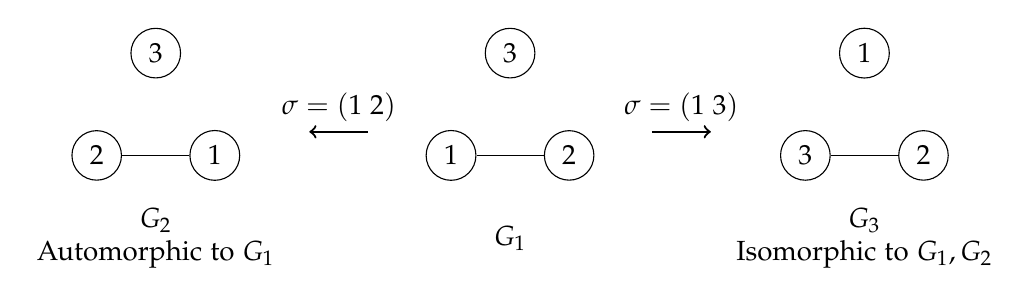
\begin{tikzpicture}[scale=1.5]
        % Graph 1
        \node[circle, draw] (g1v1) at (0, 0) {2};
        \node[circle, draw] (g1v2) at (1, 0) {1};
        \node[circle, draw] (g1v3) at (0.5, 0.866) {3};
    
        \draw[-] (g1v1) -- (g1v2);
    
        % Graph 2 (Automorphism)
        \node[circle, draw] (g2v2) at (3, 0) {1};
        \node[circle, draw] (g2v1) at (4, 0) {2};
        \node[circle, draw] (g2v3) at (3.5, 0.866) {3};
    
        \draw[-] (g2v2) -- (g2v1);
    
        % Graph 3
        \node[circle, draw] (g3v3) at (6, 0) {3};
        \node[circle, draw] (g3v2) at (7, 0) {2};
        \node[circle, draw] (g3v1) at (6.5, 0.866) {1};
    
        \draw[-] (g3v2) -- (g3v3);

        % % Arrows
        % \draw[->, thick] (g2v2) to[out=135,in=45] node[midway, above] {2 $\rightarrow$ 1} (g1v2);
        % \draw[->, thick] (g2v2) to[out=-135,in=-45] node[midway, below] {2 $\rightarrow$ 3} (g3v2);
      
        % Arrows
        \draw[<-, thick] (1.8, 0.2) -- node[midway, above] {$\sigma = (1\; 2)$} (2.3, 0.2);
        \draw[->, thick] (4.7, 0.2) -- node[midway, above] {$\sigma = (1\; 3)$} (5.2, 0.2);

    
        % Labels
        \node[align=center] at (0.5, -0.7) {$G_2$ \\Automorphic to $G_1$};
        \node[align=center] at (3.5, -0.7) {$G_1$};
        \node[align=center] at (6.5, -0.7) {$G_3$\\ Isomorphic to $G_1, G_2$};
    
    \end{tikzpicture}
    \caption{Example automorphic/isomorphic graphs}
    \label{fig:automorphic_isomorphic_graphs}
\end{figure}

To be concrete, take an example graph $G = (V, E) = (\{1, 2, 3\}, \{(1,2)\})$ which is shown as $G_1$ in \cref{fig:automorphic_isomorphic_graphs}. It's a "labelled graph". $G$ is isomorphic to any other labelled graph $H$ if they look the same if you anonymise the nodes.
More formally, if $f: V(G) \to V(H)$ is a bijection mapping nodes to nodes, such that $u \sim v$ in $G$ $\iff f(u) \sim f(v)$ in $H$, then $G$ is isomorphic to $H$, and the permutation $\sigma$ we denoted previously is precisely $f$. So $G$ is isomorphic to $H$ with edge set $\{(1, 3)\}$. You can even say that it is automorphic to the graph $H$ with edge set $\{(2, 1)\}$, i.e. just switching nodes $1,2$.
On this graph $G$ of 3 nodes, there are $3! = 6$ node ID permutations, each of which produces an isomorphic graph $G'$. For our particular $G$, we could group together these 6 isomorphic graphs $G'$ into 3 pairs of automorphic graphs.

Hence the bayesian evidence compuation is actually to sample $\theta$,  then for each $\sigma \in S_n$ create $G'$ where $G$ is isomorphic to $G'$ with permutation $sigma$ ($G \stackrel{\sigma}{\to} G'$), and calculate $p(G' | \theta)$; add these up and take the average.
Finally repeat for further $\theta$ samples and take an outer average.


Consider a simplified Chung-Lu / GIRG model where all nodes have the same weight $1$, and $\theta = (\vec{x}_1, \vec{x}_2, \vec{x}_3)$ of the three nodes. The Chung-Lu has identical $p(G')$ for each of the 6 ismorphisms. The GIRG  model does not - if $\vec{x}_1, \vec{x}_2$ are close, and $\vec{x}_3$ is far from both, then it awards higher probability to $G' = (V, \{(1,2)\})$ and $G' = (V, \{(2, 1)\})$. Furthermore both models always award the same probability to any equivalent class of automorphic graphs - this is because the adjacency matrix is the same for automorphic graphs, which is all that the models care about.

Unfortunately computing the $n!$ sized $\sum_{\sigma} p(G' \stackrel{\sigma}{\cong} G | \theta) p(\sigma)$ is infeasible for all but tiny graphs. As an alternative, we hoped to use a graph similarity kernel $k$ which compares two graphs $G, H$, giving some measure $k(G, H)$ of how similar they are up to ismorphism (in a node permutation invariant way).
Apparently one more computable example is the random walk kernel.
Therefore the idea would be to replace the incorrect $p(G | \cG_{\text{d-}\GIRG}) = \int_\theta p(G | \theta) p(\theta) d\theta$ with 
% $\mu(G) = \int_\theta k(G, G' \sim \cG_\theta) p(\theta) d\theta$. This is an idea.
$\mu(G) = E_{G' \sim \cG_{\text{d-}\GIRG}} \left [ k(G, G') \right ]$.

% Therefore the idea would be to replace the incorrect $p(G | \cG_{\text{d-}\GIRG}) = \int_\theta p(G | \theta, \cG_{\text{d-}\GIRG}) p(\theta | \cG_{\text{d-}\GIRG}) d\theta$ with $\mu(G) = E_{G' \sim \cG_{\text{d-}\GIRG}} \left [ k(G, G') \right ]$. This is an idea.

% So when we say $p(G | \theta)$, we actually mean the probability of getting a graph $G'$ which is isomorphic to $G$, given parameters $\theta$.



% TODO do we remove this weird figure - what's it doing here? 
\begin{figure}
    \centering

    \begin{subfigure}{0.49\textwidth}
      \centering
      \includegraphics[width=\linewidth]{figures/socfb-Amherst41-1d.png}
      \caption{$d=1$}
    \end{subfigure}
    \hfill
    \begin{subfigure}{0.49\textwidth}
      \centering
      \includegraphics[width=\linewidth]{figures/socfb-Amherst41-2d.png}
      \caption{$d=2$}
    \end{subfigure}
  
    \vspace{1em}
  
    \begin{subfigure}{0.49\textwidth}
      \centering
      \includegraphics[width=\linewidth]{figures/socfb-Amherst41-3d.png}
      \caption{$d=3$}
    \end{subfigure}
    \hfill
  
    \caption{MCMC runs for socfb-Amherst41, without failure rate}
    \label{fig:amherst_non_failure_mcmc}
\end{figure}

We see in \cref{fig:amherst_non_failure_mcmc} that Bayes Factor model comparison wise, 1D GIRGs are superior, even though according to edge accuracy, 2D GIRGs achieve a slight edge.


\section{Graph Kernel Introduction}
Graph Kernels provide a means for a similarity metric between graphs. They're ideally a positive semidefinite function $k: \Gamma \times \Gamma \rightarrow \mathbb{R}$, where $\Gamma$ is the set of all graphs. Such a function exists if and only if there is a corresponding feature map resentation of $\phi: \Gamma \to \cH_\phi$ where $\cH_\phi$ is a Hilbert space, and $k(G, G') = \langle \phi(G), \phi(G') \rangle_{\cH_\phi}$ is just an inner product.

Graph kernels give a simplified version of Blasius' classification framework. Blasius compares multiple different graph feature combinations on which to train an SVM for distinguishing two graph datasets. Instead we can replace this with a single kernel which hopefully encapsulates sufficient relevant information on the graph. The question of which graph features to use then shifts to which graph kernel to use!

Another benefit of graph kernels is, as a similarity metric, they give easier direct comparison between graphs.
In the previous sections' proposed paradigm, we can directly compare the similarity of a real graph $G$ with two synthetic graphs $G_1, G_2$, produced from different models $M_1, M_2$, using $k(G, G_1)$ and $k(G, G_2)$.
% This is simply done by comparing $k(G, G_1)$ and $k(G, G_2)$ - the higher of the two is the more similar.


% Graph Kernels have many uses, but we can use them in particular to help with bayesian model comparison, solving our issue of graph permutations.

% A survey on graph kernels https://appliednetsci.springeropen.com/articles/10.1007/s41109-019-0195-3



% We saw the equation $\mu(G) = E_{G' \sim \cG_{\text{d-}\GIRG}} \left [ k(G, G') \right ]$ in the previous chapter. We can Monte Carlo sample this expectation to get an estimate.

\section{Experiments with Random Walk Kernel; Weisfeiler-Lehman Kernel}
There are a range of graph kernels to choose from, however given the relatively large size of our graphs, runtime can be an issue. We ended up testing two kernels, however unfortunately both proved unsatisfactory. Without further expertise on graph kernels, we were forced to abandon this line of attack. We think that graph kernels might give more meaningful similarity metrics on smaller graphs with more unique structure (our random graph models and the real graphs themselves have a lot of homogenous structure) and particularly meangingful node labels.

\subsection{Random Walk Kernel}
The random walk kernel between two graphs is conceptually a count of the number of random walks of any length $l$ that exist in the product graph. This is generally an infinite sum, so geometric weighting with the factor $\lambda^l$ is used to decay the contribution of longer walks, where $0 < \lambda < 1$ (we tested with $\lambda=10^{-5}$).

The product graph between $G, G'$ is defined as $G_\times = (V_\times, E_\times)$ where $V_\times = \{(v, v') | v \in V, v' \in V'\}$ and $E_\times = \{((v_1, v'_1), (v_2, v'_2)) | v_1 \sim v_2 \in E_1, v'_1 \sim v'_2 \in E_2\}$. This definition can be extended to node-labelled graphs, where we only take product vertices $(v, v') \in V_\times$ if $v \in V, v' \in V'$ have the same label.

The naive implementation of the random walk kernel has complexity $O(n^6)$, however this can be sped up to $O(n^3)$. This is still too slow for our purposes. We only made limited tests with small graphs of $n \leq 3000$ nodes - see e.g. \cref{fig:rw_kernel_fitcopycube}.

\subsection{Weisfeiler-Lehman Kernel}
The Weisfeiler-Lehman kernel runs much faster in $O(h|E|)$ time, where $|E|$ is the number of edges in the graph and $h$ is the number of iterations of the algorithm. The algorithm requires some kind of node labelling - we colour nodes into a small discreet set of colours by grouping together nodes with similar sized degrees. It also uses a base kernel which is computed at each iteration - we used the simplest/speediest node label histogram dot product kernel: $k(G, G') = \langle \vec{f}, \vec{f}' \rangle$ where $\vec{f} = (f_1, \dots, f_k)$, $f_i = |\{ v \in V \;:\; l(v) = i\}|$ is the number of nodes with label $i$.

The output is $k_{WLK}(G, G') = k_{\text{base}}(G_1, G_1') + \dots + k_{\text{base}}(G_h, G_h')$. $G=G_1,\; G' = G'_1$, and $G_{i+1}$ is computed iteratively as relabelling each node in $G_i$ with $l(v) \gets (l(v), (l(u))_{u \sim v})$. This looks odd, but in practice each label is just rehashed as a new integer rather than becoming a highly nested tuple.



\subsection{Experiments}

Unfortunately both kernels failed to pass a basic test of ratifying one type of GIRG model over another. We tried a variety of combinations, but didn't get such reliable results: see \cref{fig:wl_kernel_gentorus} and \cref{fig:rw_kernel_fitcopycube}.

E.g. in \cref{fig:rw_kernel_fitcopycube}, the random walk kernel faield the basic test of having $k(G \sim \cG_1, G'_1 \sim \cG_1) > k(G \sim \cG_1, G'_2 \sim \cG_2)$, where $\cG_1$ is a 3D copy weight cube GIRG, and $\cG_2$ is copy weight Chung-Lu.

\begin{figure}
  \centering
\includegraphics[width=0.8\linewidth]{figures/d=2 alpha=1.2 n=70000 GIRG WL-Kernel with others.png}
\caption{WL-Kernel of a d=2, alpha=1.2, n=70000 Torus GIRG with other generated graphs (13 per model). All the GIRGs are more similar to the original than Chung-Lu, but we cannot differentiate between GIRGs of different dimensions.}
\label{fig:wl_kernel_gentorus}
\end{figure}

% socfb-Brandeis99 d=3.png


\begin{figure}
  \centering
\includegraphics[width=0.8\linewidth]{figures/socfb-Brandeis99 d=3.png}
\caption{RW-Kernel of a d=3 copy weight cube GIRG fit to socfb-Brandeis99 (matching number of edges and local clustering coefficient), with other generated graphs (6 per model type). Chung-Lu graphs have highest similarity to the original, despite it being a 3D GIRG}
\label{fig:rw_kernel_fitcopycube}
\end{figure}



% We think that 


% \subsection{Experiments}
% we do the comparison

% Cube Similarity Plots:
% We fit alpha, c for a uniform cube GIRG for dimensions d=1-3, produce a graph, and look at similarity with real graph.


\chapter{Conclusion}
The goal of this thesis was to explore the capacity of different GIRG model variants to match real social network graphs, due to their suspected inherent geometrical generation and power law tailed degree distribution. In documenting our various experiments, we also detailed our methods and ideas for working with GIRGs and graph data which may prove useful to other practitioners.

Our first achievement was to follow the realism framework of \cite{blasius2018towards}, to compare a range of generative graph models, including many GIRG subtypes, in their ability to replicate global statistics of a set of 104 social network graphs.
Our results showed that GIRGs showed superior performance in replicating several key statistics: node closeness centralities, node betweenness centralities, effective graph diameter, and mean local clustering coefficient. We identified variations between different GIRG subtypes, with max norm cube GIRGs excelling at diameter replication, MCD GIRGs on closeness centrality, and max norm torus GIRGs on betweenness centrality. 
Interestingly, increasing the geometric dimension did not yield significant improvements, indicating that 1-3 dimensions might be adequate to achieve a high-level similarity to real-world graphs. 1d often proved best, however mixed min/max GIRGs demonstrated good performance while having higher dimensionality, they should be explored further along with distorted GIRGs.

Subsequently, we explored fitting GIRG node geometric location parameters to real-world social network graphs, to see if GIRGs are capable of exact replication of them on a node and edge level. This proved quite successful, showing that GIRGs can capture a high percentage of edges, even with just 1 dimension. Adding further dimensions is computationally intensive and doesn't increase the fit substantially. Our range of fitting methods might be further refined in practice according to the use case. 

The different GIRG variants that we have covered have only recently risen to prominence, and future work might explore and compare them more thoroughly. In particular, the mixed min/max GIRGs and distorted GIRGs are promising. On the practical side, other real graph datasets than the Facebook social networks we used might be explored, and particularly ones with node attributes that really provide a ground truth geometry. Whether they can be well fit by GIRGs using methods similar to ours would be fascinating. Adapting the GIRG uniform location priors and power law weight priors to something more flexible and realistic could also be a fruitful avenue of research.


\paragraph{Many thanks} to my supervisors Marc Kaufmann and Ulysse Schaller, as well as Johannes Lengler and Afonso Bandeira, for their valuable input and guidance throughout the thesis. Thank you to Angelika Steger and her lab for their friendly and welcoming research environment. Finally much appreciation to friends, family, ETH, etc. for their support and existence. And thank you to the reader for making it this far! I hope it has been an enjoyable / interesting read.




% \begin{figure}
%   \centering
% \includegraphics[width=0.8\linewidth]{figures/d=2 alpha=1.2 n=70000 GIRG WL-Kernel with others.png}
% \caption{WL-Kernel of a d=2, alpha=1.2, n=70000 Torus GIRG with other generated graphs (13 per model). All the GIRGs are more similar to the original than Chung-Lu, but we cannot differentiate between different GIRGs.}
% \label{fig:wl_kernel_gentorus}
% \end{figure}

% socfb-Brandeis99 d=3.png


% \begin{figure}
%   \centering
% \includegraphics[width=0.8\linewidth]{figures/socfb-Brandeis99 d=3.png}
% \caption{RW-Kernel of a d=3 copy weight cube GIRG fit to socfb-Brandeis99 (matching number of edges and local clustering coefficient), with other generated graphs (6 per model type). Chung-Lu graphs have highest similarity to the original, despite it being a 3D GIRG}
% \label{fig:rw_kernel_fitcopycube}
% \end{figure}




% \appendix

% \input{appendix}

\backmatter

\bibliographystyle{apalike}
\bibliography{refs}

\includepdf[pages={-}]{declaration-originality.pdf}

\end{document}
